\chapter{Polynomial Trajectory Optimization}\label{sec:trajectory}


\section{Polynomial Trajectory}\label{sec:polynomial}

Regarding the differentiability of polynomials, they are a profound choice to represent a trajectory, especially for the use in a differentially flat representation of the UAV dynamics. (Flatness in the proper sense of system theory means that all the states and inputs can be expressed in terms of the flat output and a finite number of its derivative).
Furthermore, the differentiability of polynomials enables the possibility to check the derivatives of the trajectory for bounding violations to avoid input saturation. This saturation-check can be performed during trajectory optimization and therefore guarantees the feasibility of the resulting trajectory.

\section{Optimization}\label{sec:optimization}

The goal of this master thesis is to optimize a trajectory which passes through waypoints (also called vertices or nodes) which are defined in advance. This waypoints can be chosen manually or by a path-finding algorithm such as RRT* which will be discussed in chapter \ref{chap:RRT}.
Furthermore, not only the waypoints (i.e. the position) can be fixed in advance but also its derivatives (such as speed, acceleration etc.). The position and its derivatives are then utilized as the equality constraints for a QP (explained in Section \ref{sec:quadratic}).

\subsection{Cost Function}\label{sec:cost}

Optimization for the purpose of trajectory planning means to minimize a cost function. The cost function in this case is a combination of temporal and geometric cost. The geometric cost penalizes the square of the derivatives of the trajectory. In this master thesis the geometric cost is represented by the squared snap which guarantees a trajectory without abrupt  control inputs. \newline
The temporal cost is simply the total trajectory time multiplied by a user chosen factor $k_T$ which determines the aggressiveness of the resulting trajectory. The impact of  $k_T$  can be seen in equation \ref{equ:total_cost} which represents the combined geometric and temporal cost. \newline

To express the geometric cost in a compact way one can utilize the Hessian matrix $Q$. The Hessian matrix is defined as a squared matrix of second-order partial derivatives which follows from differentiation a function with respect to each of its coefficients, in this instance the polynomial coefficients. The geometric cost function $J(T)$ for one segment with the duration $T$ can now be written as

\begin{equation}
J(T)  = p^T \cdot Q(T) \cdot p
\end{equation}

where $Q(T)$ is the Hessian matrix for a fixed segment time $T$. $p$ is the vector containing the coefficients of the polynomial trajectory. \newline

If the trajectory consists of more than one segment the Hessian matrix has to be extended to a block-diagonal matrix. The geometric cost function for multiple segments with fixed but individual segment times $T_i$ can be written as

\begin{equation}
J(T) =
\begin{bmatrix}
   p_1 \\
\vdots \\
  p_n
\end{bmatrix}^T
\cdot
\begin{bmatrix}
   Q_1(T_1) &  &  \\
    & \ddots &  \\
   & & Q_n(T_n)
\end{bmatrix} 
\cdot
\begin{bmatrix}
   p_1 \\
\vdots \\
  p_n
\end{bmatrix}
\label{equ:cost}
\end{equation}


\subsection{Polynomial Optimization as a Constrained QP}

The cost function in equation \ref{equ:cost} has to be minimized under constraints since we want to fix things like start or end position. In a first intuitive approach the constraints on the endpoint derivatives are utilized in a constrained QP. Therefore, a mapping matrix $E$ between endpoint derivatives and polynomial coefficients is needed. The resulting equality constraint for the $i^{th}$ segment can be written as

\begin{equation}
E_i \cdot p_i = d_i
\label{equ:mapping}
\end{equation}

where $p$ is the vector containing the polynomial coefficients and $d$ is the vector containing the endpoint derivatives. Regarding the total number of segments of the trajectory, equation \ref{equ:mapping} can be written in matrix form:

\begin{equation}
\begin{bmatrix}
   E_1 &  &  \\
    & \ddots &  \\
   & & E_n
\end{bmatrix} 
\cdot
\begin{bmatrix}
   p_1 \\
\vdots \\
  p_n
\end{bmatrix}
=
\begin{bmatrix}
   d_1 \\
\vdots \\
  d_n
\end{bmatrix}
\end{equation} 

The constrained QP is suitable for a small amount of segments but gets ill-conditioned for a large amount of segments and therefore large matrices. Especially if there are matrices which are close to singularity and have coefficients which are close to zero, the constrained QP can get numerical unstable.

\subsection{Polynomial Optimization as a Unconstrained QP}\label{sec:polynomialQP}

To avoid the numerical instability of a constrained QP the optimization problem is converted into a unconstrained QP. To achieve this, the polynomial coefficients $p_i$ from equation \ref{equ:cost} have to be substituted by the endpoint derivatives $d_i$ which are now the new optimization variables. The cost function of the unconstrained QP can now be written as 

\begin{equation}
J =
\begin{bmatrix}
   d_1 \\
\vdots \\
  d_n
\end{bmatrix}^T
\cdot
\begin{bmatrix}
   E_1 &  &  \\
    & \ddots &  \\
   & & E_n
\end{bmatrix} ^{-T}
\cdot
\begin{bmatrix}
   Q_1 &  &  \\
    & \ddots &  \\
   & & Q_n
\end{bmatrix} 
\cdot
\begin{bmatrix}
   E_1 &  &  \\
    & \ddots &  \\
   & & E_n
\end{bmatrix} ^{-1}
\cdot
\begin{bmatrix}
   d_1 \\
\vdots \\
  d_n
\end{bmatrix}
\label{equ:uncon_cost}
\end{equation}

where $Q_i$ is the Hessian matrix according to the $i^{th}$ segment time $T_i$.\newline

As mentioned above, the endpoint derivatives are the new optimization variables. Due to the equality constraints some of the endpoint derivatives are already specified consequently reducing the number of optimizations variables. Expediently, the endpoint derivatives are divided in fixed derivatives $d_f$ and unspecified derivatives $d_p$ and then reordered using the matrix $C$ which consists of zeros and ones. After reordering the endpoint derivatives equation \ref{equ:uncon_cost} can be rewritten as

\begin{equation}
J =
\begin{bmatrix}
   d_f \\
  d_p
\end{bmatrix}^T
\underbrace{C^T E^{-T} Q E^{-1} C}_\text{R}
\begin{bmatrix}
   d_f \\
  d_p
\end{bmatrix}
\label{equ:R_cost}
\end{equation}

where the product of the reordering matrix $C$, the mapping matrix $E$ and the Hessian matrix $Q$ can be expressed as a single Matrix $R$. The matrix $R$ for his part can be divided into four submatrices according to the fixed and unspecified endpoint derivatives which modifies equation \ref{equ:R_cost} as follows:

\begin{equation}
J =
\begin{bmatrix}
   d_f \\
  d_p
\end{bmatrix}^T
\begin{bmatrix}
   R_{ff} & R_{fp} \\
  R_{pf} & R_{pp}
\end{bmatrix}
\begin{bmatrix}
   d_f \\
  d_p
\end{bmatrix}
\label{equ:Rxx_cost}
\end{equation}

Partially differenting equation \ref{equ:Rxx_cost} with respect to the unspecified derivatives $d_p$ and equate it to zero yields the optimized/minimized unspecified derivatives $d_p^*$ 

\begin{equation}
d_p^* = - R_{pp}^{-1} \cdot R_{fp}^T \cdot d_f
\label{equ:dpstar}
\end{equation}

as a function of the fixed derivatives $d_f$ and two of the submatrices ($R_{pp}, R_{fp}$) of $R$. Equation \ref{equ:dpstar} can now be used to compute the initial solution. 


\section{Initial Solution}\label{sec:initialSolution}

As can be seen in equation \ref{equ:uncon_cost}, the Hessian matrix for the  $ i^{th}$ segment $Q_i$ depends on the segment time $T_i$. Thus, all the segment times have to be defined in advance. For the initial solution the segment times are calculated based on the Euclidean distance $d_{norm}$ and on the user specified maximal speed ($v_{max}$) and maximal acceleration ($a_{max}$). \newline

Basically, the segment time is determined by the term $d_{norm}/v_{max} \cdot 2$ which is twice the time the UAV would need for a segment by flying the whole distance at maximal speed. Although this is a good estimation for long segments, for shorter ones the time needed to accelerate gets significant. In order to incorporate acceleration time, a multiplier which is zero for long segments and larger than zero for short ones is added. The segment time $T_i$ for the $i^{th}$ segment can be computed according to 

\begin{equation}
T_i = \frac{d_{norm_i}}{v_{max}} \cdot 2 \cdot \left( 1 + 6.5 \cdot \frac {v_{max}}{a_{max}} \cdot \frac{1}{e^{\frac{d_{norm_i}}{v_{max}} \cdot 2}} \right)
\label{equ:segmentTime}
\end{equation}

where $d_{norm_i}$ is the Euclidean distance of the $i^{th}$ segment, $v_{max}$ the user specified maximal velocity and $a_{max}$ the user specified maximal acceleration. The fraction $v_{max}/a_{max}$ gives an idea of how much time is needed to accelerate to maximum velocity whereas $6.5$ is a empirical weighting factor. \newline

The result of equation \ref{equ:segmentTime} is depicted in figure \ref{pic:timeEstimation} whereat the $x$-axis represents the Euclidean distance $d_{norm}$ and the $y$-axis represents the segment time $T$. For this plot the user specified limitation on speed has been set to $v_{max} = 3 \frac{m}{s}$  and the limitation on acceleration has been set to  $a_{max} = 5 \frac{m}{s^2}$. The dashed green line represents the term $d_{norm}/v_{max} \cdot 2$ and serves as a reference. The blue graph is the exact representation of equation \ref{equ:segmentTime}. 

\begin{figure}[H]
   \centering
   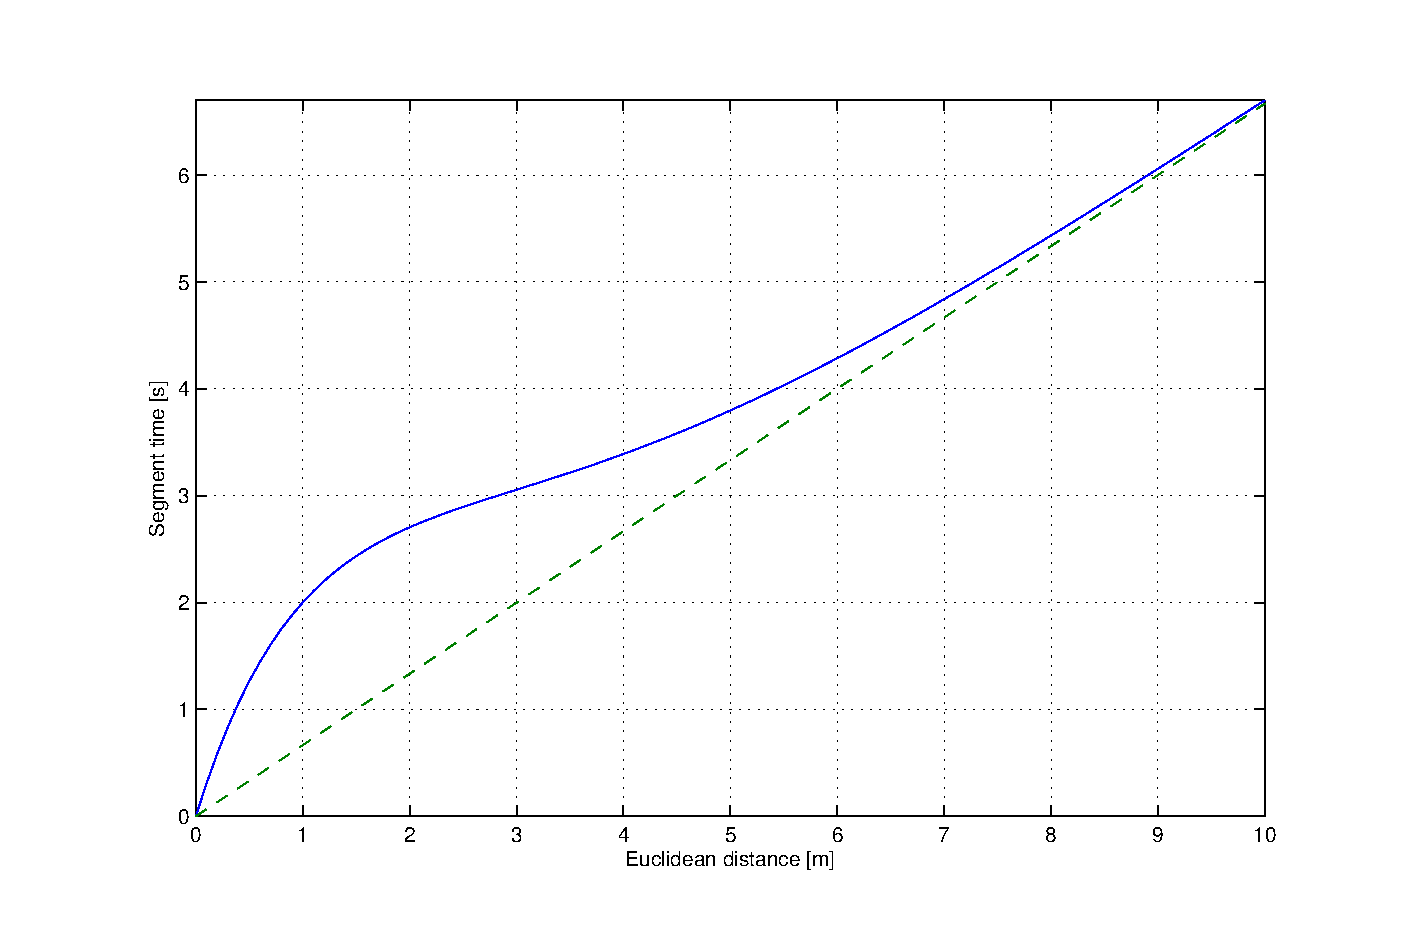
\includegraphics[trim = 20mm 10mm 20mm 10mm,width=1\textwidth]{pics/time_estimation.eps}
   \caption{The segment time $T$ depends on the Euclidean distance $d_{norm}$ of a segment as well as on the max. velocity $v_{max}$ and the max. acceleration $a_{max}$. Integration of acceleration time has an impact on segment time for short distances.}
   \label{pic:timeEstimation}
\end{figure}

Once the segment times are calculated, the initial snap minimized solution can be computed according to equation \ref{equ:dpstar}. The initial solution for a 3 dimensional problem with 2 segments is depicted in figure \ref{pic:initialSolution}. The start of the trajectory is the origin of the Cartesian coordinate system (0/0/0). For both, start and goal state, the velocity, the acceleration, the jerk and the snap are fixed and set to zero. For all the other sampling points (vertices) the derivatives are unspecified. The Cartesian coordinates of the sampling points are chosen manually and are listed in the following table.  For the sake of convenience, a simple set of vertex with coordinates which increase permanently have been chosen:

\begin{table}[H] 
\begin{center}
    \begin{tabular}{ | l | c | c | c |}
    \hline
    Waypoint & x-coordinate & y-coordinate & z-coordinate\\ \hline
    Start-Vertex & 0 & 0 & 0 \\ \hline
    Vertex 1 & 1 & 2 & 5\\ \hline
    Goal-Vertex & 3 & 4 & 6\\
    \hline
    \end{tabular}
    \caption{3 manually chosen  vertices.}
    \label{tab:vertices}
\end{center}
\end{table}


The initial solution depicted in figure \ref{pic:initialSolution} is divided into 3 plots. Plot a) shows the position (i.e. the Cartesian coordinates) whereby each of the 3 dimensions is depicted as a single graph. The Cartesian coordinates from the above-noted table are depicted as circles. 
Plot b) shows the velocity of the individual direction as a solid graph. Additional, the velocity in the three-dimensional space (i.e. the Euclidean norm of the velocity vector) is depicted as a dashed graph.
Plot c) depicts the acceleration in the individual directions (solid) and the acceleration in the three-dimensional space (dashed). Furthermore the limitation for velocity and acceleration ($v_{max} = 3 \frac{m}{s}$ and $a_{max} = 4 \frac{m}{s^2}$ for this problem) are depicted in plot b) resp. c) . The $x$-axis for all the 3 plots is the time. \newline


\begin{figure}[h]
   \centering
   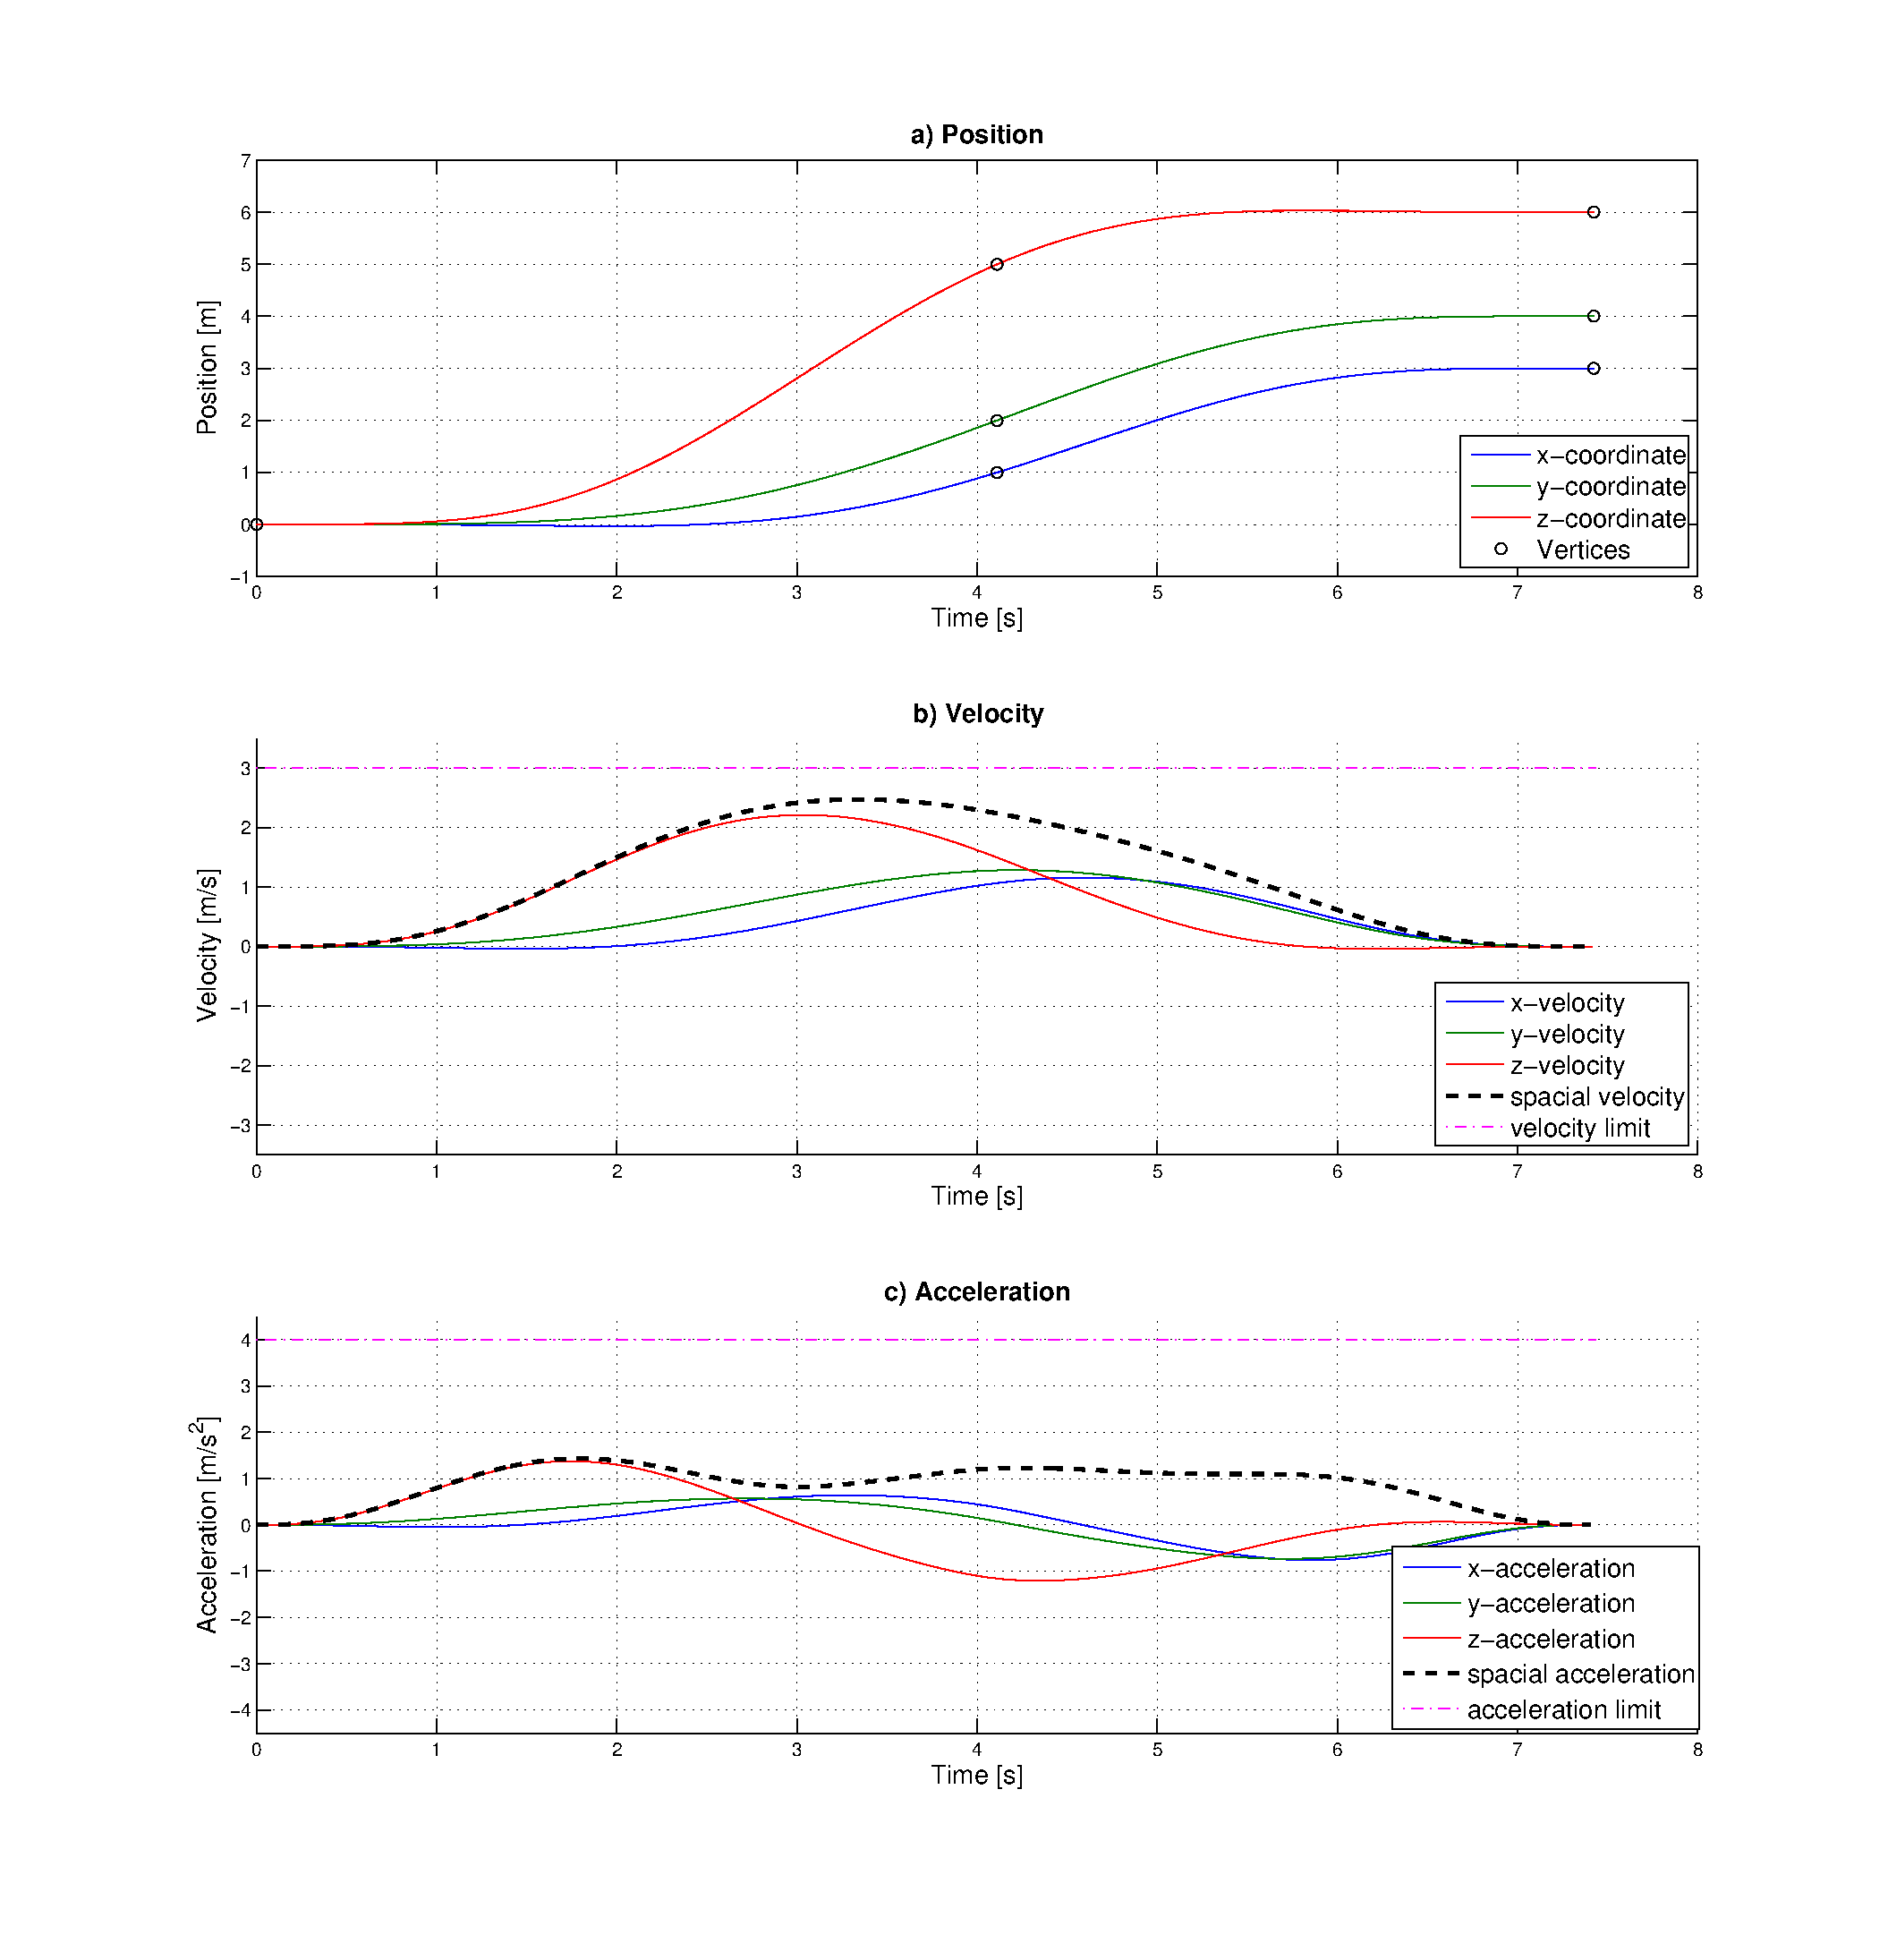
\includegraphics[trim = 32mm 30mm 30mm 20mm,clip,width=0.984\textwidth]{pics/2SegInit7s43.eps}
   \caption{Initial solution of a trajectory with 2 segments: Plot a) shows the position (i.e. the Cartesian coordinates). Plot b) shows the velocity and plot c) the acceleration. A dashed graph represents the velocity respectively the acceleration in the three-dimensional space.}
   \label{pic:initialSolution}
\end{figure}

As can be seen in plot b) the maximal spacial velocity is less then the user specified maximal velocity $v_{max} = 3\frac{m}{s}$. The same applies to plot c) where the maximal acceleration is far below the user specified maximal acceleration of $a_{max} = 4 \frac{m}{s^2}$. Hence, the trajectory could be more aggressive/faster without violating the limitations. \newline

\subsection{Drawbacks of the Initial Solution}\label{sec:drawbackInitial}


The individual segment times and consequently the total time of the initial trajectory are defined by equation \ref{equ:segmentTime}. Since equation \ref{equ:segmentTime} does not incorporate the circumstances from one segment to another it is likely to find a better trajectory (i.e. a trajectory with a smaller total cost) with the same total time but a different ratio between the segment time. Moreover, there is no possibility to adjust the aggressiveness of the initial solution since the segment times are calculated up-front. \newline

In summary, the modification of the individual segment times and therefore the modification of the ratio of the segment times can lead to a solution with smaller cost. Supplementary, the modification of the individual segment times gives us the opportunity to adjust the aggressiveness of a trajectory.



\section{Time Allocation}\label{sec:penalty}

So fare, only the geometric cost (i.e. the squared snap) was included in the cost function defined in equation \ref{equ:Rxx_cost}. Minimization of the geometric cost ensures a smooth trajectory without abrupt input signal but has no effect on the aggressiveness of a trajectory. Therefore equation \ref{equ:Rxx_cost} has to be extended by the temporal cost (i.e. the sum of the segment times) which results in the total cost $J_{total}$

\begin{equation}
J_{total} =
\begin{bmatrix}
   d_f \\
  d_p
\end{bmatrix}^T
\begin{bmatrix}
   R_{ff} & R_{fp} \\
  R_{pf} & R_{pp}
\end{bmatrix}
\begin{bmatrix}
   d_f \\
  d_p
\end{bmatrix}
+ k_T \cdot \sum_{i=1}^N T_i
\label{equ:total_cost}
\end{equation}

where $k_T$ is a user specified weighting factor and $T_i$ is the segment time of the $i^{th}$ segment. \newline

A hight value for $k_T$ lays weight to the temporal cost and therefore leads to a trajectory with a short total trajectory time. A small value for $k_T$ on the other hand lays little weight on the temporal cost, meaning the geometric cost gets more important. Since the geometric cost (i.e. the quadratic snap) decreases for long segment times with little changes in jerk, this leads to a trajectory with a long total trajectory time. Thus, the user specified weighting factor $k_T$ enables the adjustment of the aggressiveness of a trajectory. \newline

\subsection{Nonlinear Optimization}\label{sec:nonlinearopt}

The geometric cost function in equation \ref{equ:Rxx_cost} has only the unspecified endpoint derivatives $d_p$ as optimization variables. This optimization problem can be solved analytically as performed in equation \ref{equ:dpstar}. The cost function in equation \ref{equ:total_cost} has the segment times $T_i$ as additional optimization variables, meaning the segment times $T_i$ are directly represented in the cost function and not only indirectly via the Hessian matrices $Q_{T_i}$. Since the segment times are now optimization variables, the Hessian matrices $Q_{T_i}$ are no longer defined in advance and the problem cannot be solved analytically. Due to that a nonlinear solver is used. In this master thesis NLopt, a open-source library for nonlinear optimization, is applied. The unspecified endpoint derivatives $d_p$ and the segment times $T_i$ of the initial solution are the initial values for the nonlinear solver. Meaning the initial solution has to be computed in advance to start a nonlinear optimization. \newline

To illustrate the nonlinear optimization, the trajectory with the same 3 vertices (defined in the table  \ref{tab:vertices}) is reused. In this master thesis position, velocity, acceleration, jerk and snap are fixed for the start and for the goal vertex since we want to start from complete rest and want to end up in standstill. For the vertex in the middle the position is fixed but velocity, acceleration, jerk and snap are unspecified, resulting in the first 4 optimization variables. Since this is a 3 dimensional problem, the number of geometric optimization variables triples to 12. Together with the segment time of the two segments, the problem ends up with a total number of 14 optimization variables. \pagebreak 

The result of the nonlinear optimization is depicted in figure \ref{pic:optimizedSolution}. Plot a) depicts the position (i.e. the Cartesian coordinates) whereby each of the 3 dimensions is depicted as a single graph. Plot b) shows the velocity of the individual direction as a solid graph. Additional, the velocity in the three-dimensional space (i.e. the Euclidean norm of the velocity vector) is depicted as a dashed graph. Plot c) depicts the acceleration in the individual directions (solid) and the acceleration in the three-dimensional space (dashed). Furthermore the limitation ($v_{max} = 3 \frac{m}{s}$ and $a_{max} = 4 \frac{m}{s^2}$ for this problem) are depicted. In contrast to figure \ref{pic:initialSolution}, the $x$-axis of figure \ref{pic:optimizedSolution} stops at $7s$ since the optimized trajectory is faster.
%\vspace*{3\baselineskip}

\begin{figure}[h]
   \centering
   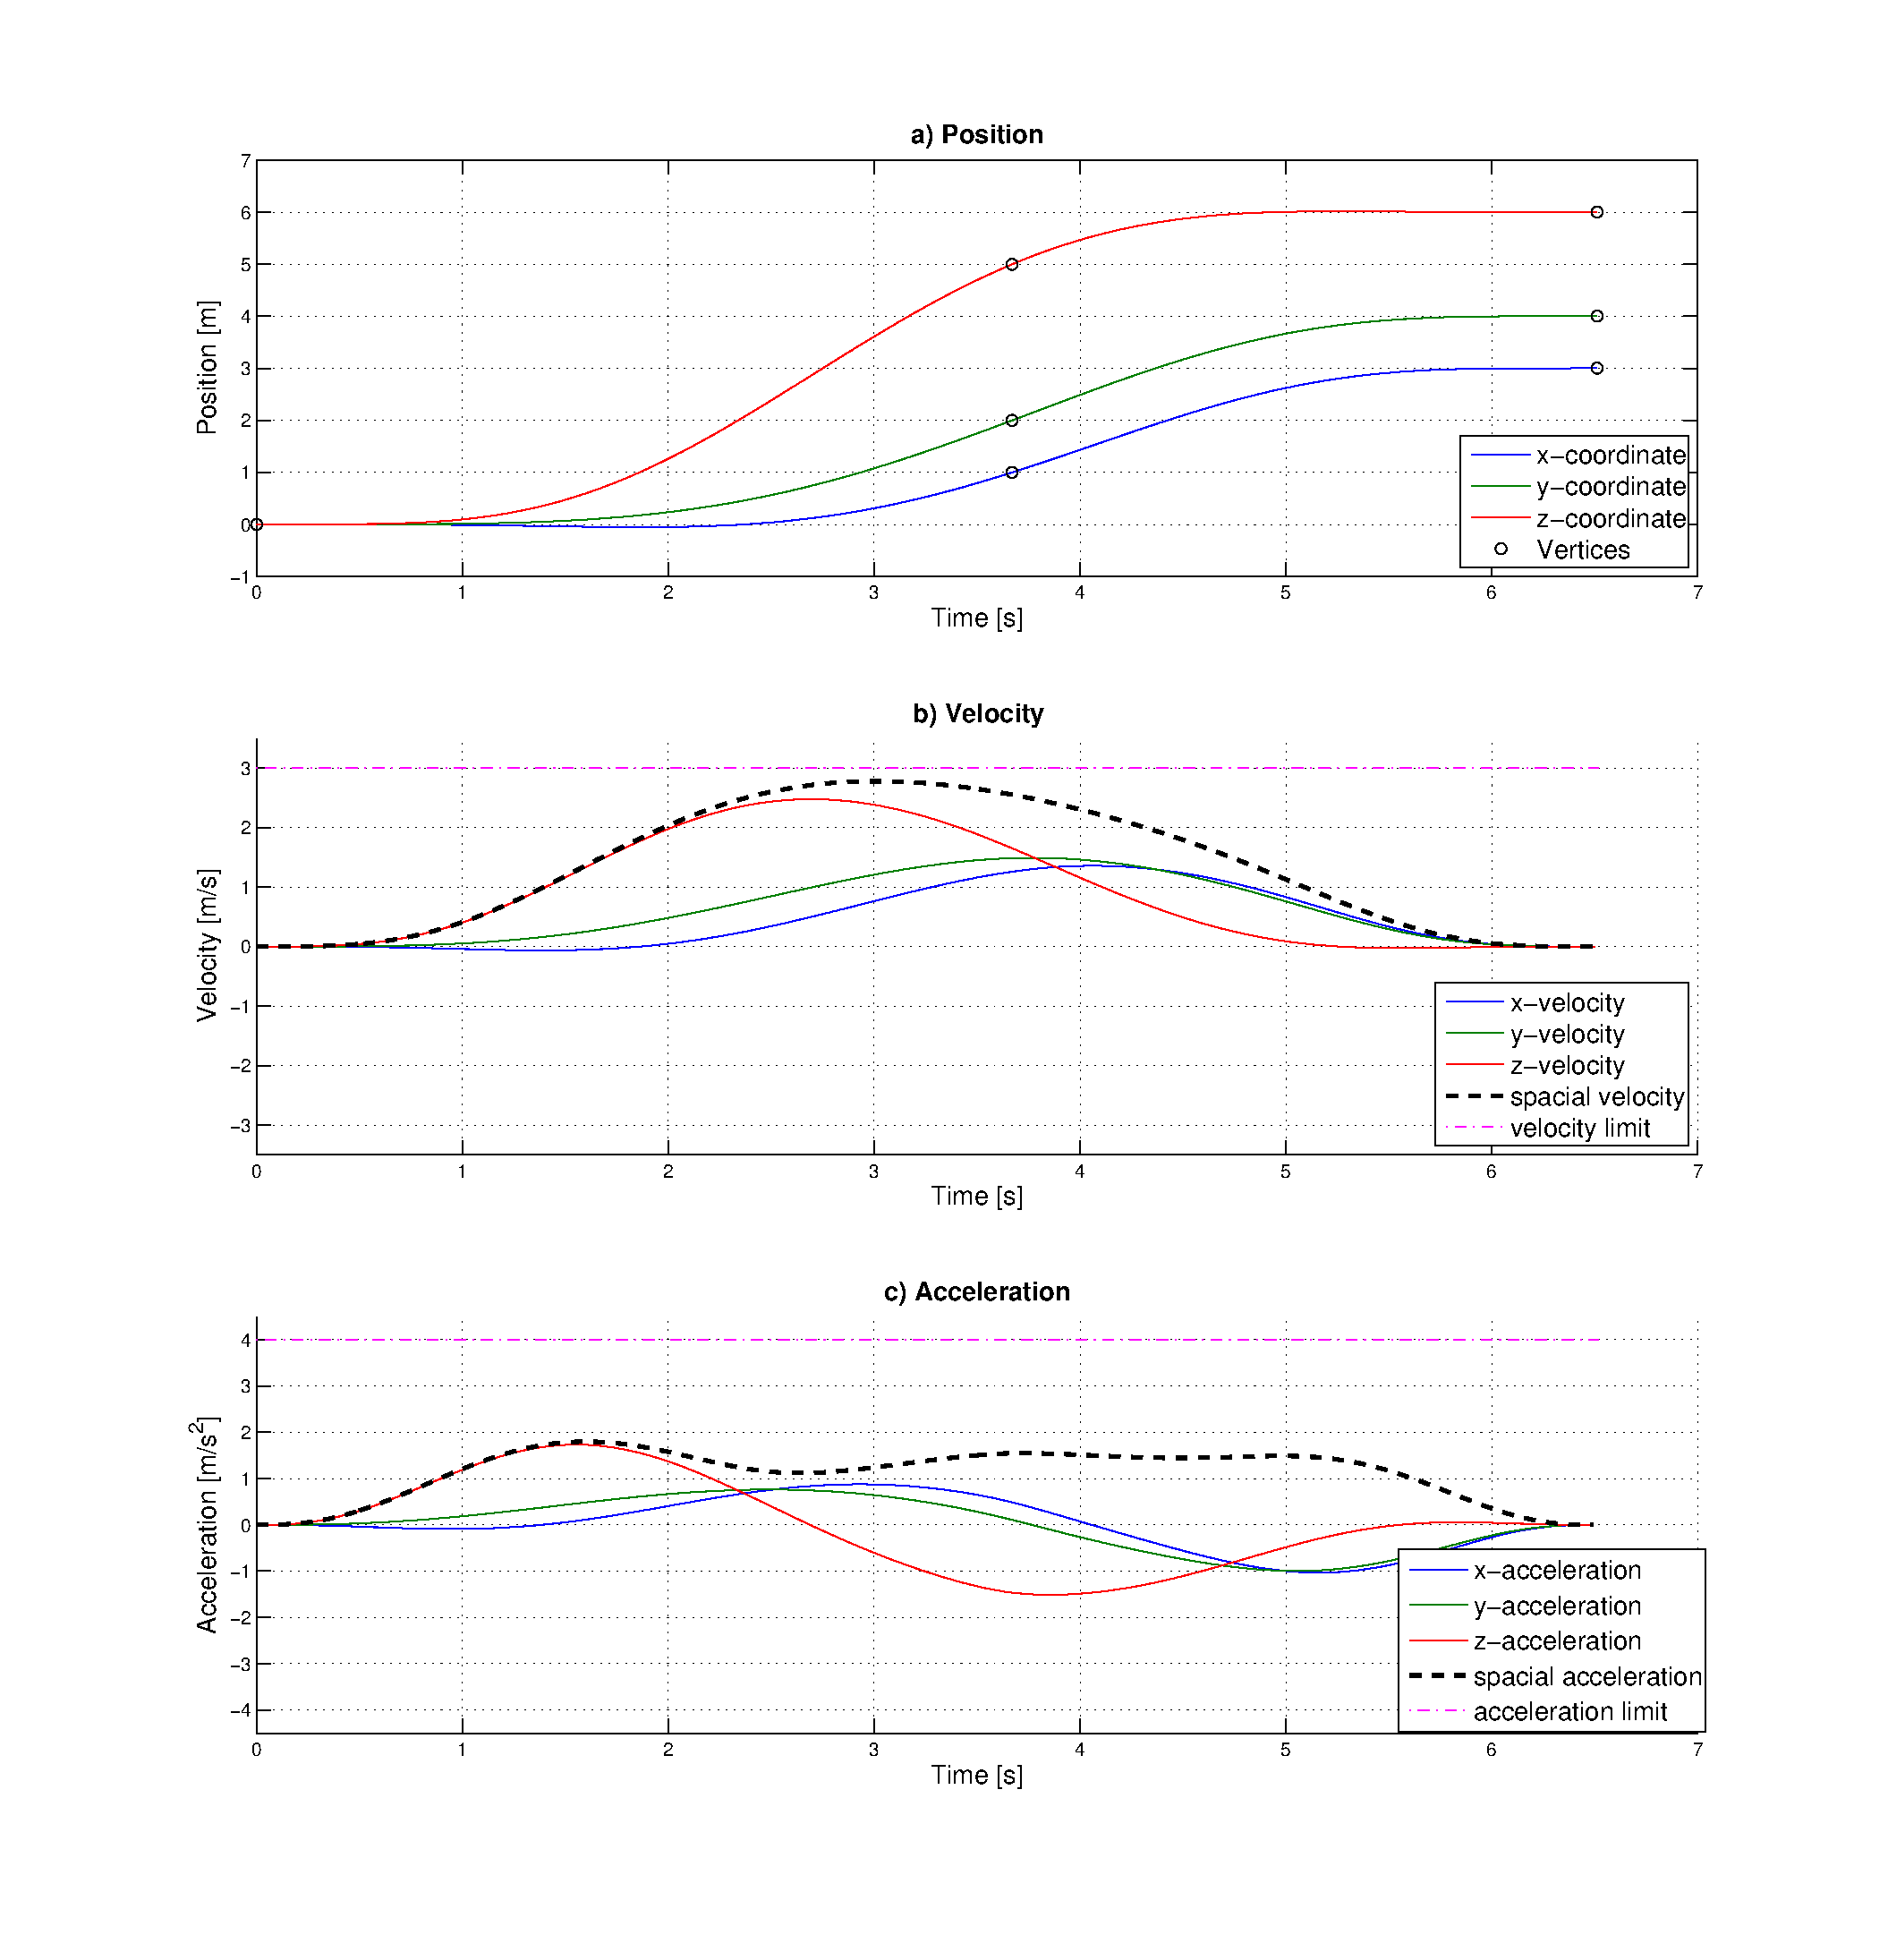
\includegraphics[trim = 33mm 20mm 30mm 8mm,clip,width=1\textwidth]{pics/2SegOpti6s52k100.eps}
   \caption{Optimized solution of a trajectory with 2 segments: Plot a) shows the position (i.e. the Cartesian coordinates). Plot b) shows the velocity and plot c) the acceleration. A dashed graph represents the velocity respectively the acceleration in the three-dimensional space. Weighting factor $k_T$ was set to 100.}
   \label{pic:optimizedSolution}
\end{figure}



As can be seen in figure \ref{pic:optimizedSolution} a) the trajectory passes the same vertices as in figure \ref{pic:initialSolution}. 
In this optimization the user specified weighting factor was set to $k_T = 100$. This rather small value for $k_T$ leads to a trajectory which is neither affected by the limitation on the velocity (the spacial velocity in plot b) is always below the velocity limit) nor by the limitation on acceleration(the spacial acceleration in plot c) is always below the acceleration limit). Nevertheless, the optimized trajectory with a duration of $6.52 s$ is faster then the initial solution with a duration of $7.43 s$.\newline

To get a more aggressive trajectory the value for $k_T$ has to be increased. In figure \ref{pic:optimizedSolution2k190} the optimize trajectory for $k_T = 190$ is depicted. As can be seen in plot b) the limitation on the velocity comes into play, i.e. the spacial velocity is restricted to $v_{max} = 3 \frac{m}{s}$. The duration of the trajectory depicted in figure \ref{pic:optimizedSolution2k190} is $6.01s$. Although the maximal velocity and the maximal acceleration are higher than in figure \ref{pic:optimizedSolution}, the pathway of the spacial velocity and of the spacial acceleration look very similar for $k_T = 100$ and $k_T = 190$.
%\vspace*{3\baselineskip}

\begin{figure}[H]
   \centering
   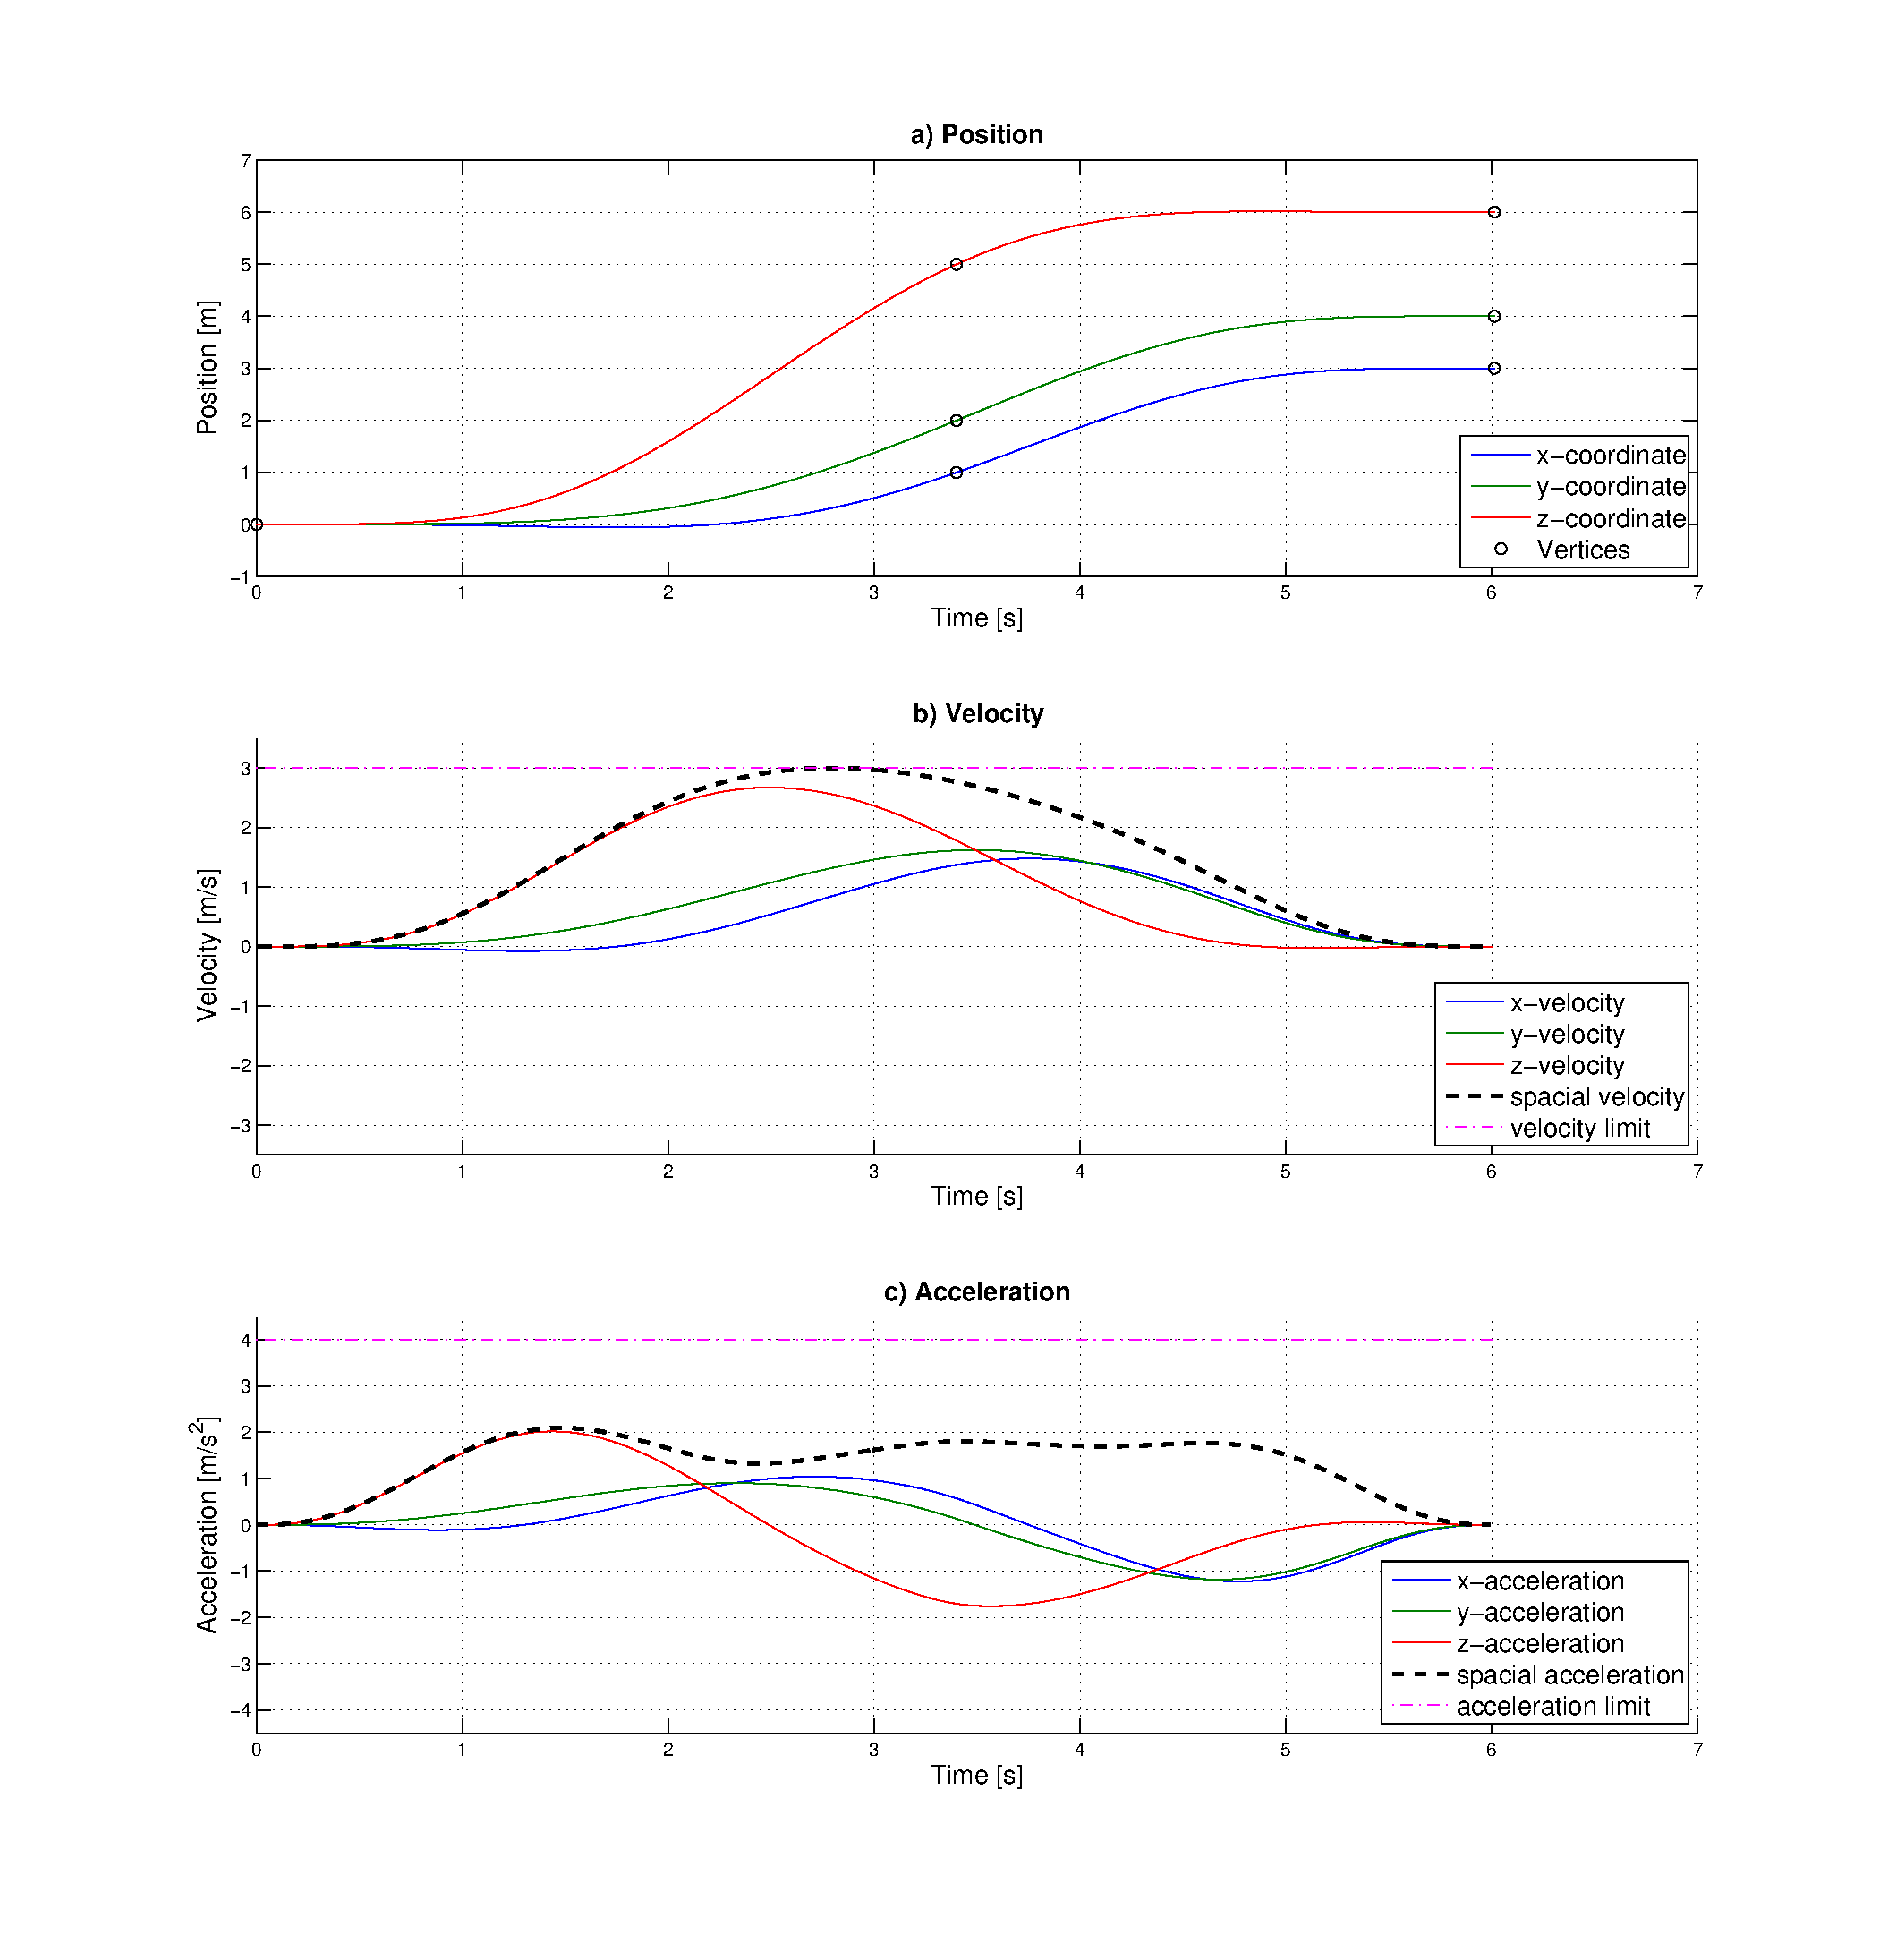
\includegraphics[trim = 33mm 20mm 30mm 15mm,clip,width=1\textwidth]{pics/2SegOpti6s01k190.eps}
   \caption{Optimized solution of a trajectory with 2 segments: Plot a) shows the position (i.e. the Cartesian coordinates). Plot b) shows the velocity and plot c) the acceleration. A dashed graph represents the velocity respectively the acceleration in the three-dimensional space. Weighting factor $k_T$ was set to 190.}
   \label{pic:optimizedSolution2k190}
\end{figure}


In a next step the value for $k_T$ is increased even more and set to $k_T = 2000$. The resulting trajectory is depicted in figure \ref{pic:optimizedSolution2k2000}. The duration of this aggressive trajectory is $5.16s$. The pathway of the spacial velocity looks now different than in the previous figures. The spacial velocity not only touches the velocity limit but stays at the limit for about one second.
%\vspace*{3.2\baselineskip}

\begin{figure}[H]
   \centering
   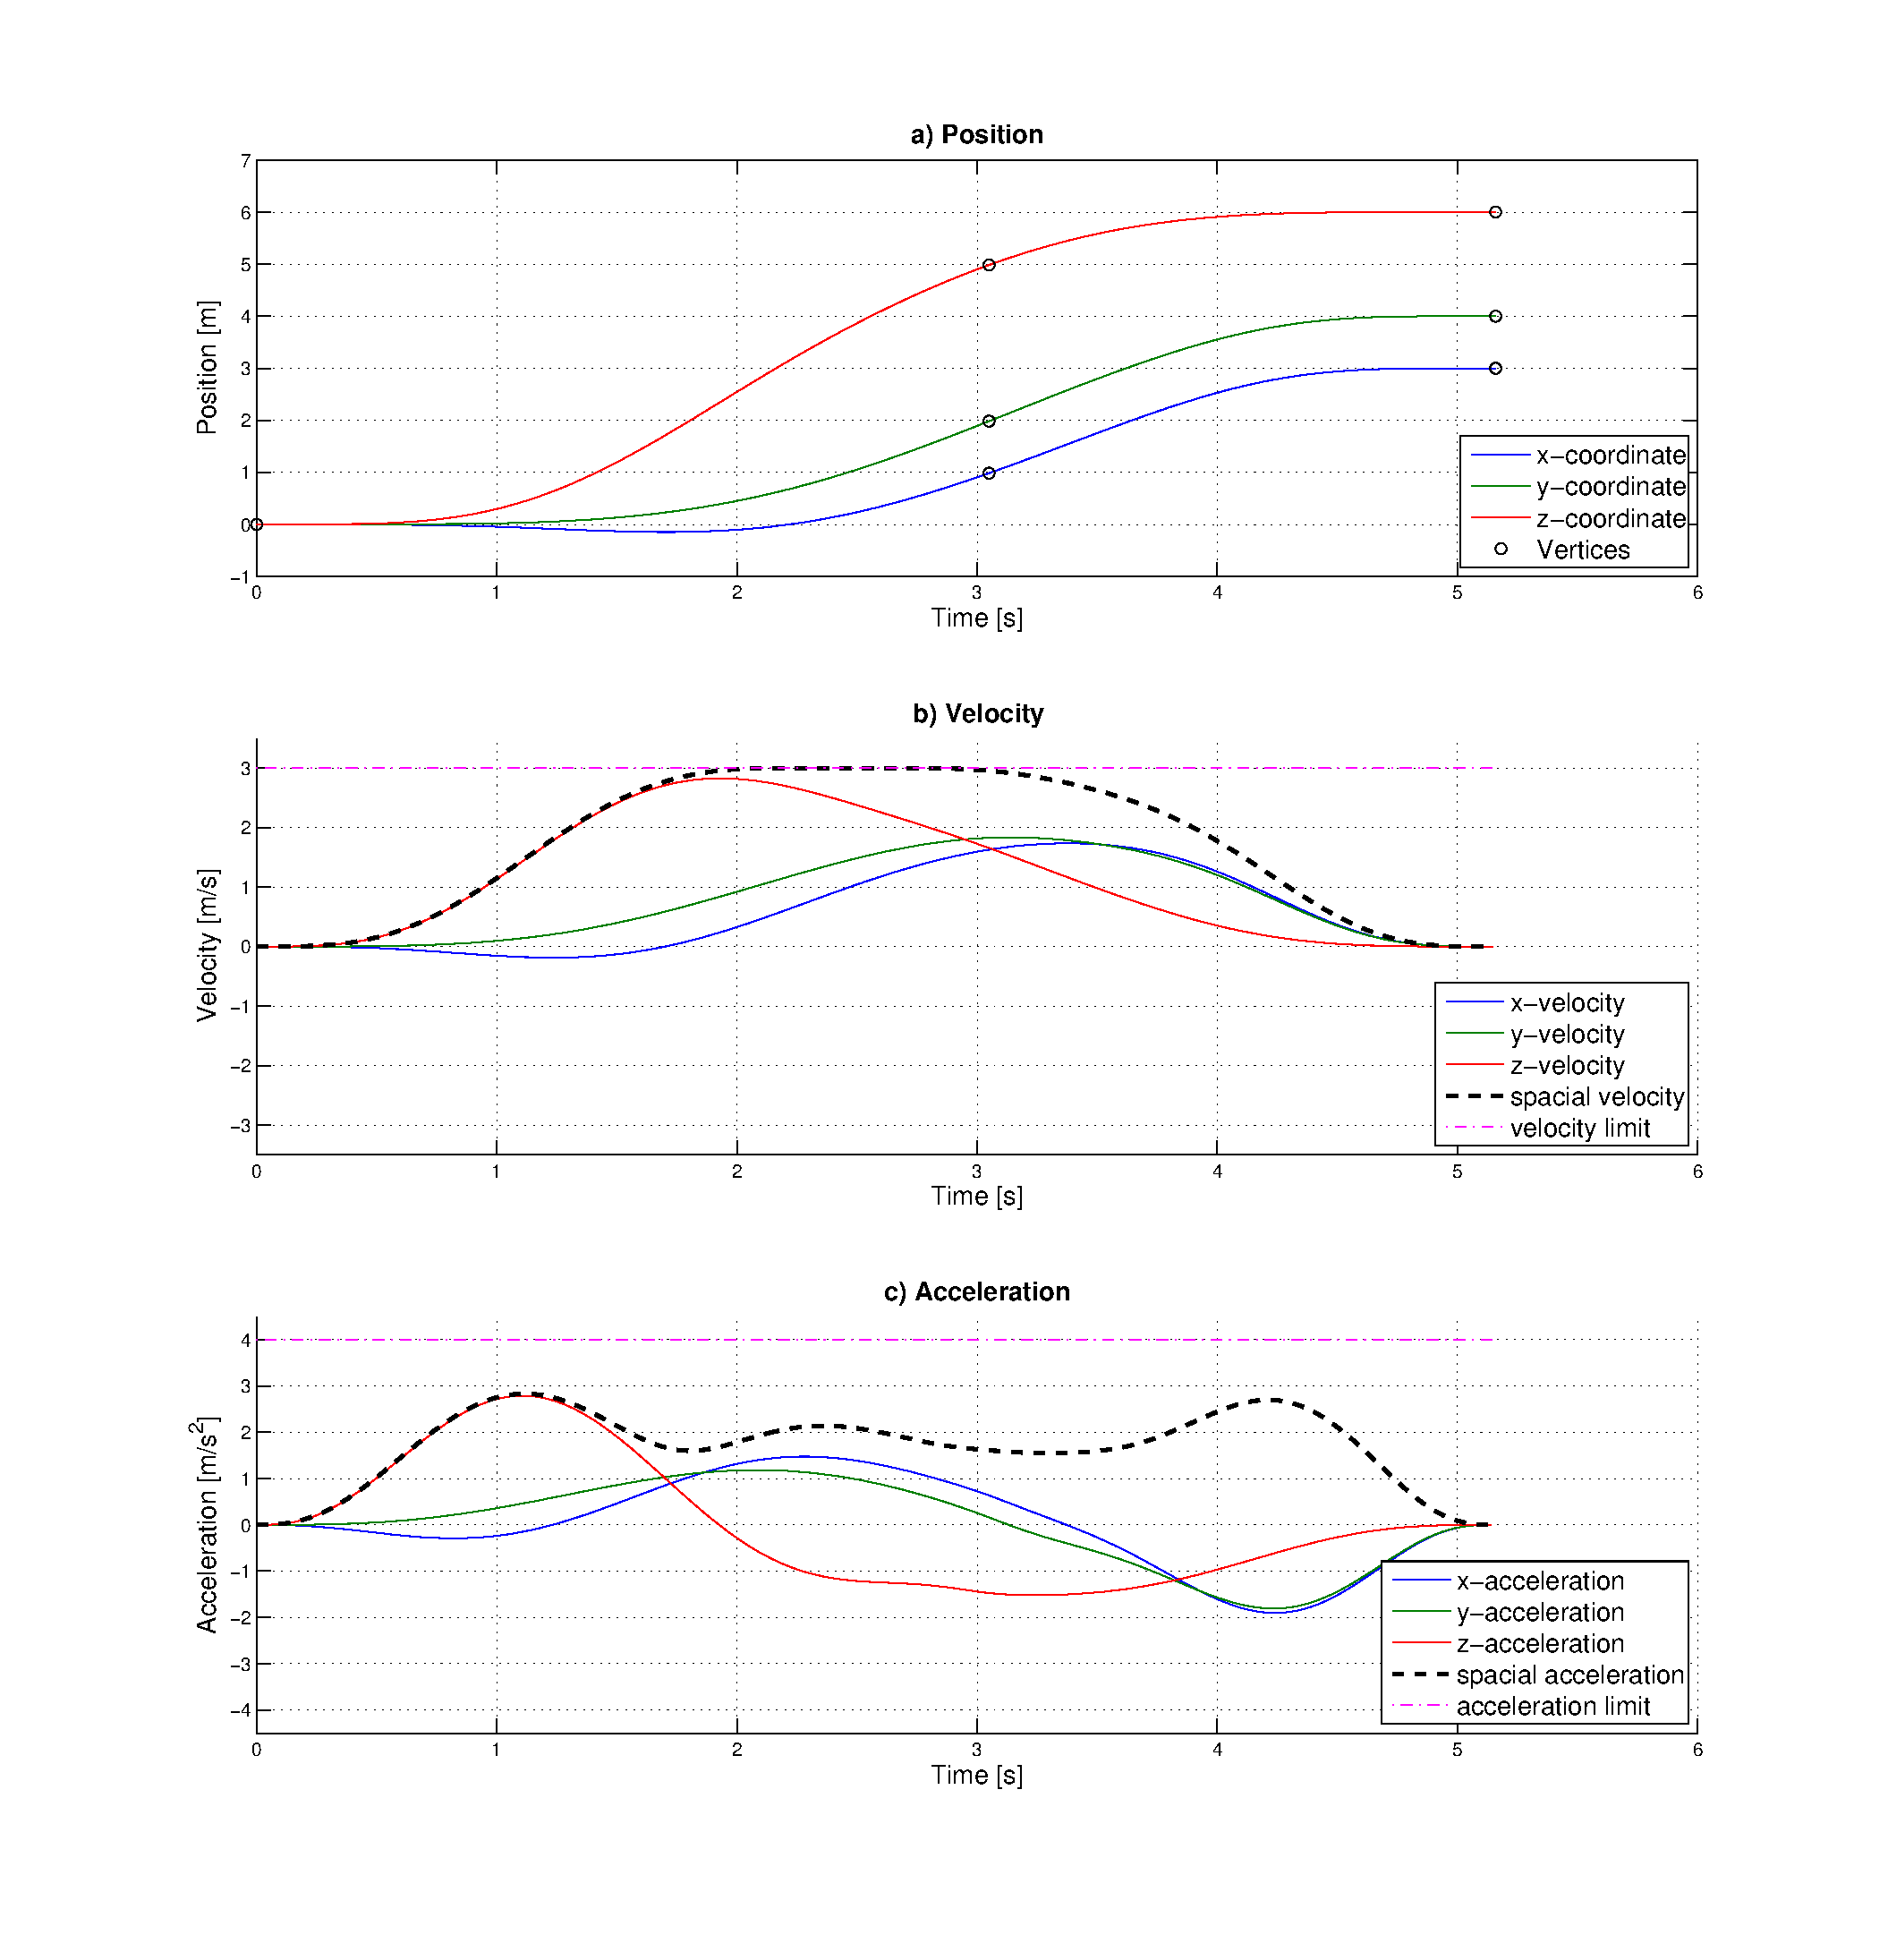
\includegraphics[trim = 33mm 30mm 30mm 15mm,clip,width=1\textwidth]{pics/2SegOpti5s16k2000.eps}
   \caption{Optimized solution of a trajectory with 2 segments: Plot a) shows the position (i.e. the Cartesian coordinates). Plot b) shows the velocity and plot c) the acceleration. A dashed graph represents the velocity respectively the acceleration in the three-dimensional space. Weighting factor $k_T$ was set to 2000.}
   \label{pic:optimizedSolution2k2000}
\end{figure}


Although figure \ref{pic:optimizedSolution2k2000} depicts an aggressive trajectory the spacial acceleration always remains under the acceleration limit. Of course this depends on the choice of the acceleration limit, i.e. the acceleration limit would get significant if $a_{max}$ is set to less than $3 \frac{m}{s^2}$.
A factor which is independent from the user specified choice of $k_T$ is the pathway of the trajectory. For a trajectory with little curves the acceleration has a smaller influence on the duration than the velocity. Since the coordinates in all 3 dimensions increase permanently, this is the case in figure \ref{pic:optimizedSolution2k2000}. \newline



To depict the features of a trajectory with more curves, a new set of vertices is chosen manually:

\begin{table}[H] 
\begin{center}
    \begin{tabular}{ | l | c | c | c |}
    \hline
    Waypoint & x-coordinate & y-coordinate & z-coordinate\\ \hline
    Start-Vertex & 0 & 0 & 0 \\ \hline
    Vertex 1 & 5 & 1 & -2\\ \hline
   Vertex 2 & 3 & -2 & 1\\ \hline
   Vertex 3 & -1 & 2 & 3\\ \hline
    Goal-Vertex & 1 & -1 & -2\\
    \hline
    \end{tabular}
\caption{5 manually chosen  vertices.}
    \label{tab:5vertices}
\end{center}
\end{table}


The initial solution with 4 segments passing through the above-noted vertices is depicted in figure \ref{pic:optimizedSolution4init}. Please note that the user specified limitation on the velocity is set to $v_{max} = 4 \frac{m}{s^2}$ for this example.


\begin{figure}[H]
   \centering
   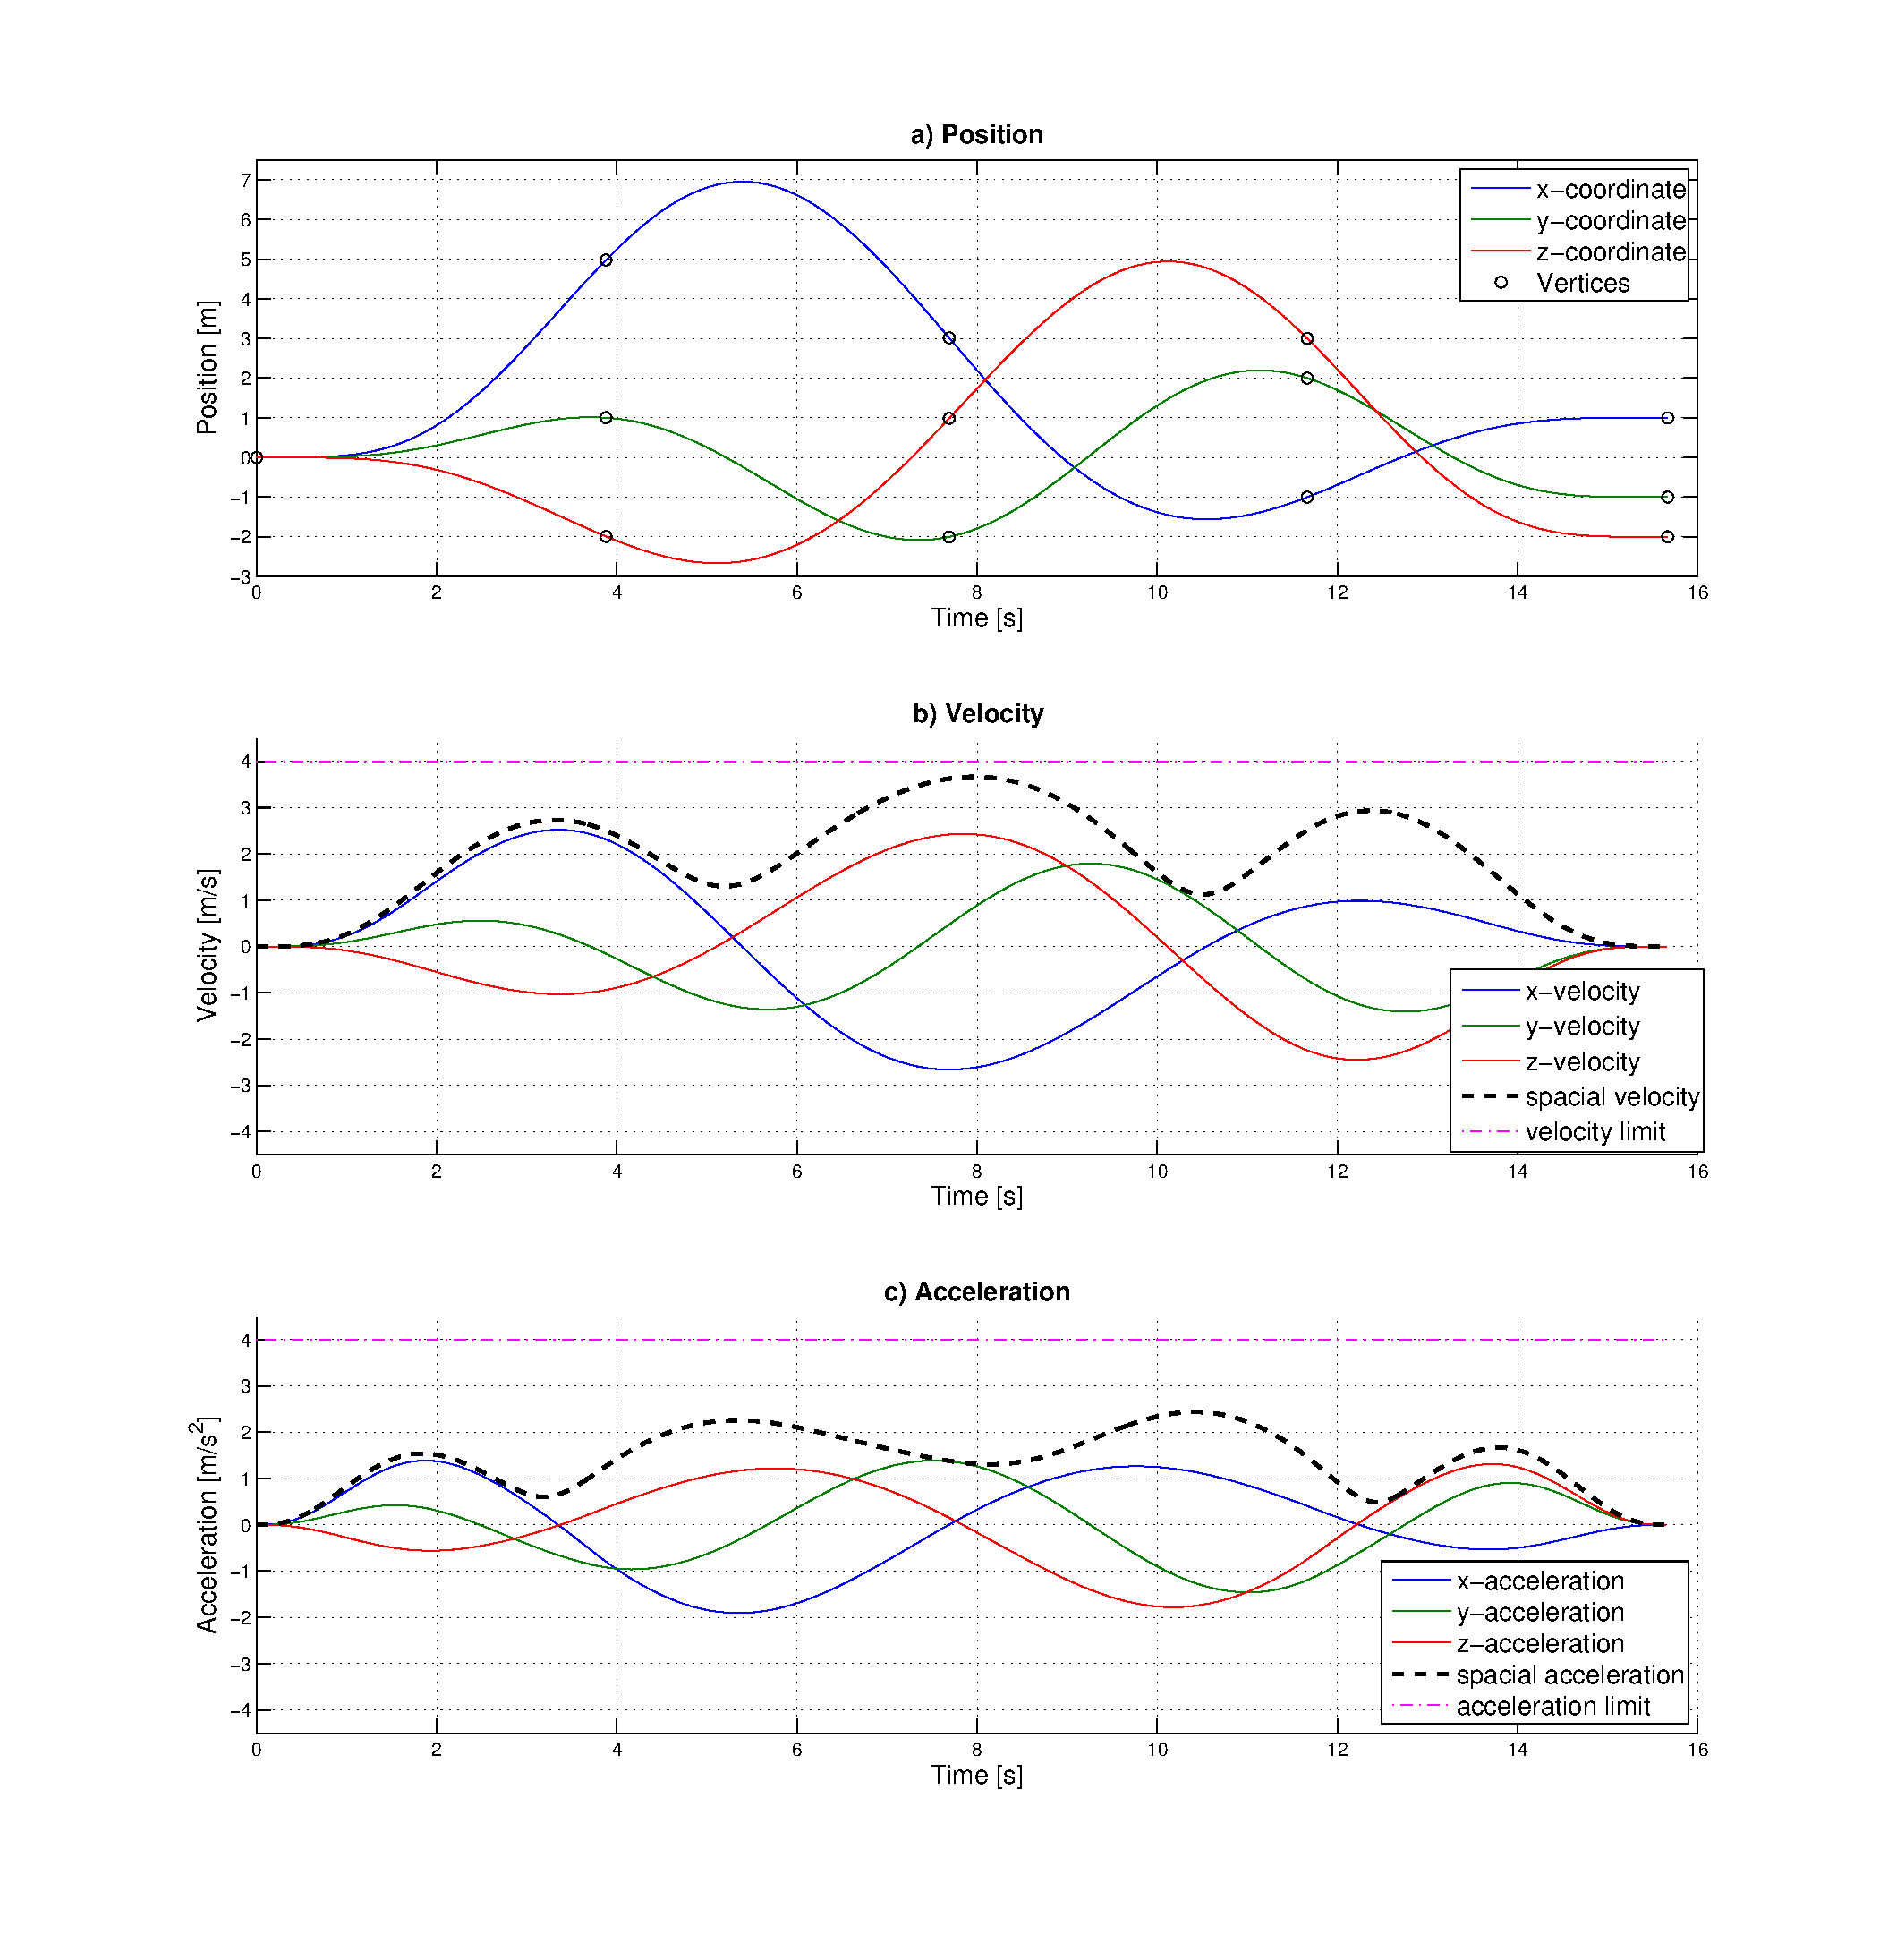
\includegraphics[trim = 33mm 30mm 30mm 15mm,clip,width=1\textwidth]{pics/4SegInit15s67.eps}
   \caption{Initial solution of a trajectory with 4 segments: A dashed graph represents the velocity respectively the acceleration in the three-dimensional space.}
   \label{pic:optimizedSolution4init}
\end{figure}
\newpage

The initial solution is required to define the initial values of the nonlinear optimization.
As can be seen in plot b) and plot c) neither the limitation on the velocity nor the limitation on the acceleration are violated.

%\begin{figure}[h]
%   \centering
%   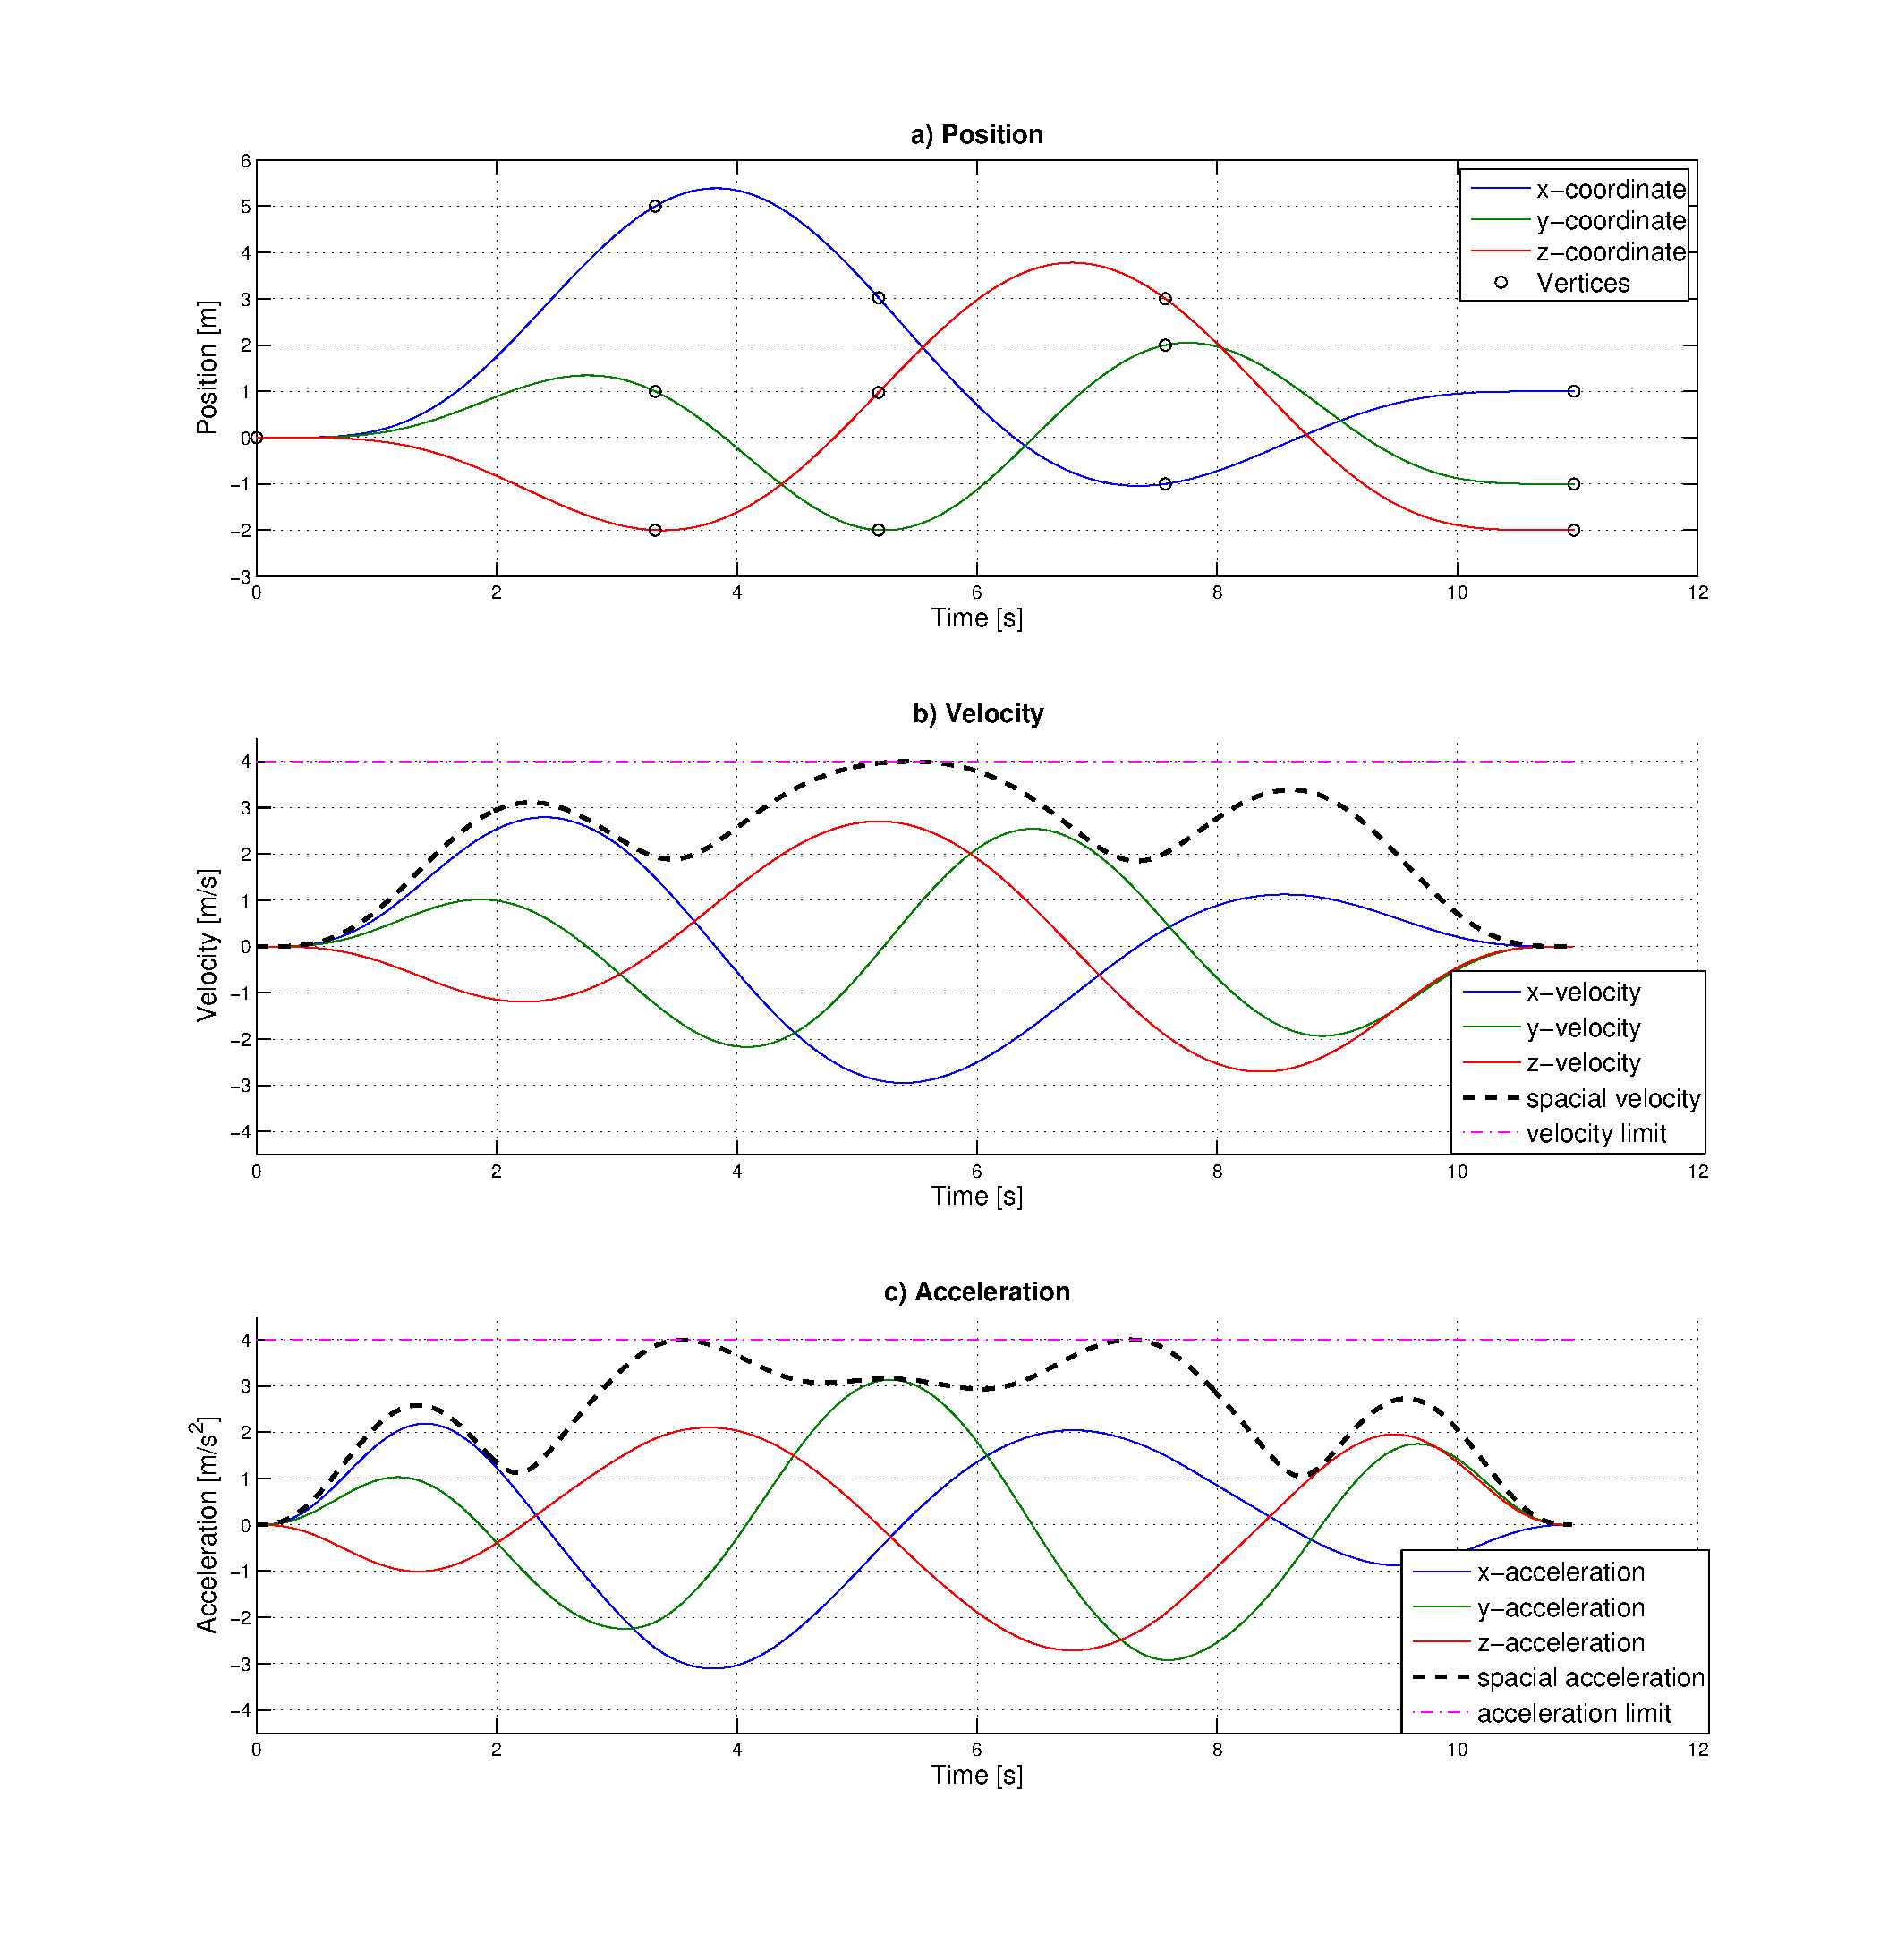
\includegraphics[trim = 35mm 20mm 30mm 35mm,width=1\textwidth]{pics/4SegOpti10s97k400.eps}
%   \caption{...................................................................................... ..... ............. . . . . ...................... ......... .........}
%\end{figure}


Using the unspecified enpoint derivatives $d_P$ and the segment times $T_i$ of the initial solution as initial values for the optimization variables the nonlinear optimization was performed with a weighting factor of $k_T = 2000$. The optimized trajectory is depicted in figure \ref{pic:optimizedSolution4optik2000}. The duration of the optimized trajectory is $10.02s$ compared to the initial trajectory duration of $15.67s$ depicted in figure \ref{pic:optimizedSolution4init}.




\begin{figure}[H]
   \centering
   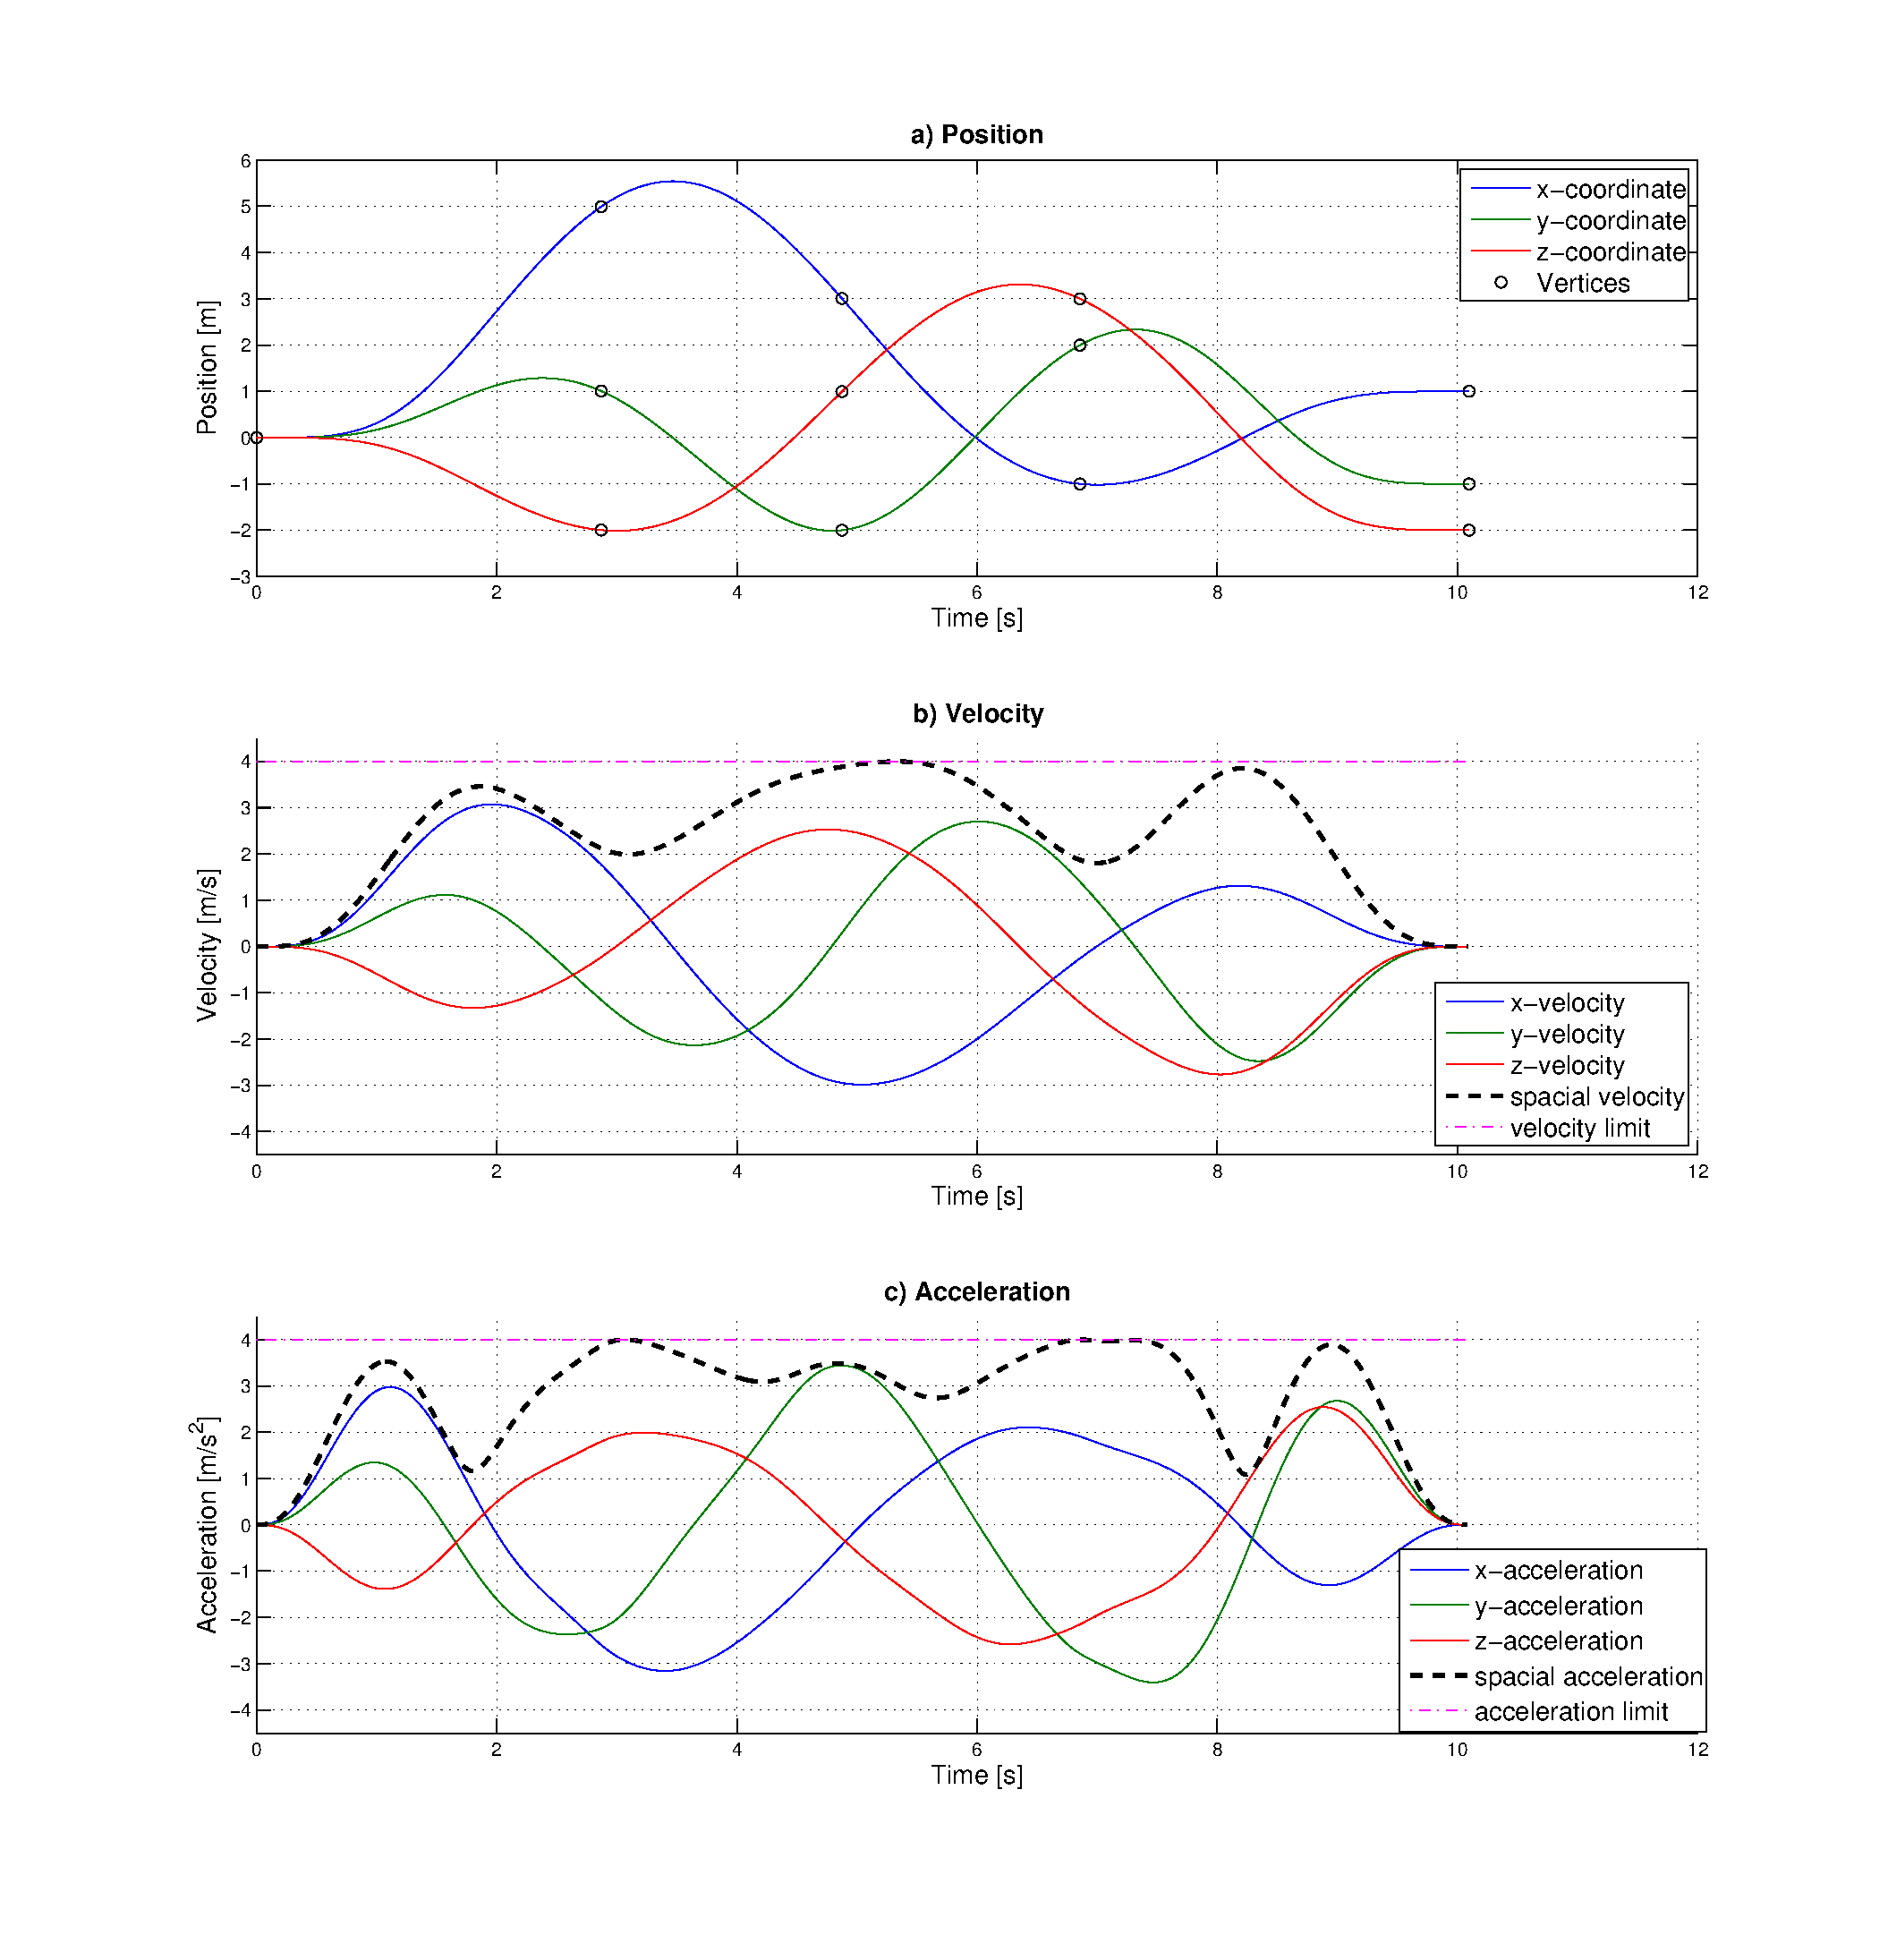
\includegraphics[trim = 33mm 30mm 30mm 15mm,clip,width=1\textwidth]{pics/4SegOpti10s01k2000.eps}
   \caption{Optimized solution of a trajectory with 4 segments: A dashed graph represents the velocity respectively the acceleration in the three-dimensional space. Weighting factor $k_T$ was set to 2000.}
   \label{pic:optimizedSolution4optik2000} 
\end{figure}

In contrast to the aggressive trajectory depicted in figure \ref{pic:optimizedSolution2k2000}, the acceleration limit has an impact on the optimized winding trajectory in figure \ref{pic:optimizedSolution4optik2000}. As can be seen in plot c) the spacial acceleration touches the acceleration limit repeatedly and even stays at exact $4 \frac{m}{s^2}$ for some time. 

\section{Pathway of the Trajectory}\label{sec:pathway}

The pathway of a snap minimized trajectory is mainly determined by the ratio of the segment times and not by the segment times themselves or by the total trajectory time. As mentioned in section \ref{sec:drawbackInitial}, the segment times from the initial solution do not consider the circumstances from one segment to an other. Hence, it is likely to find a better trajectory by changing the ratio between the segment times, even if the total time of the trajectory stays the same.

The process of optimizing the ratio of the segment times is implicitly performed during the process of nonlinear optimization. In other words, the nonlinear optimization not only changes the total trajectory time according to the weighting factor $k_T$ but also optimizes the ratio of the segment times. \newline
Such a change in the pathway is distinguishable between the initial trajectory in figure \ref{pic:optimizedSolution4init} a) and the optimized trajectory in figure \ref{pic:optimizedSolution4optik2000} a). The easiest notable difference is the peak of the $x$ graph with a peak value of 6.95 in the initial trajectory and a peak value of 5.58 in the optimized trajectory. However, the changes in the pathway are more apparent in a 3D plot. 


\begin{figure}[H]
   \centering
   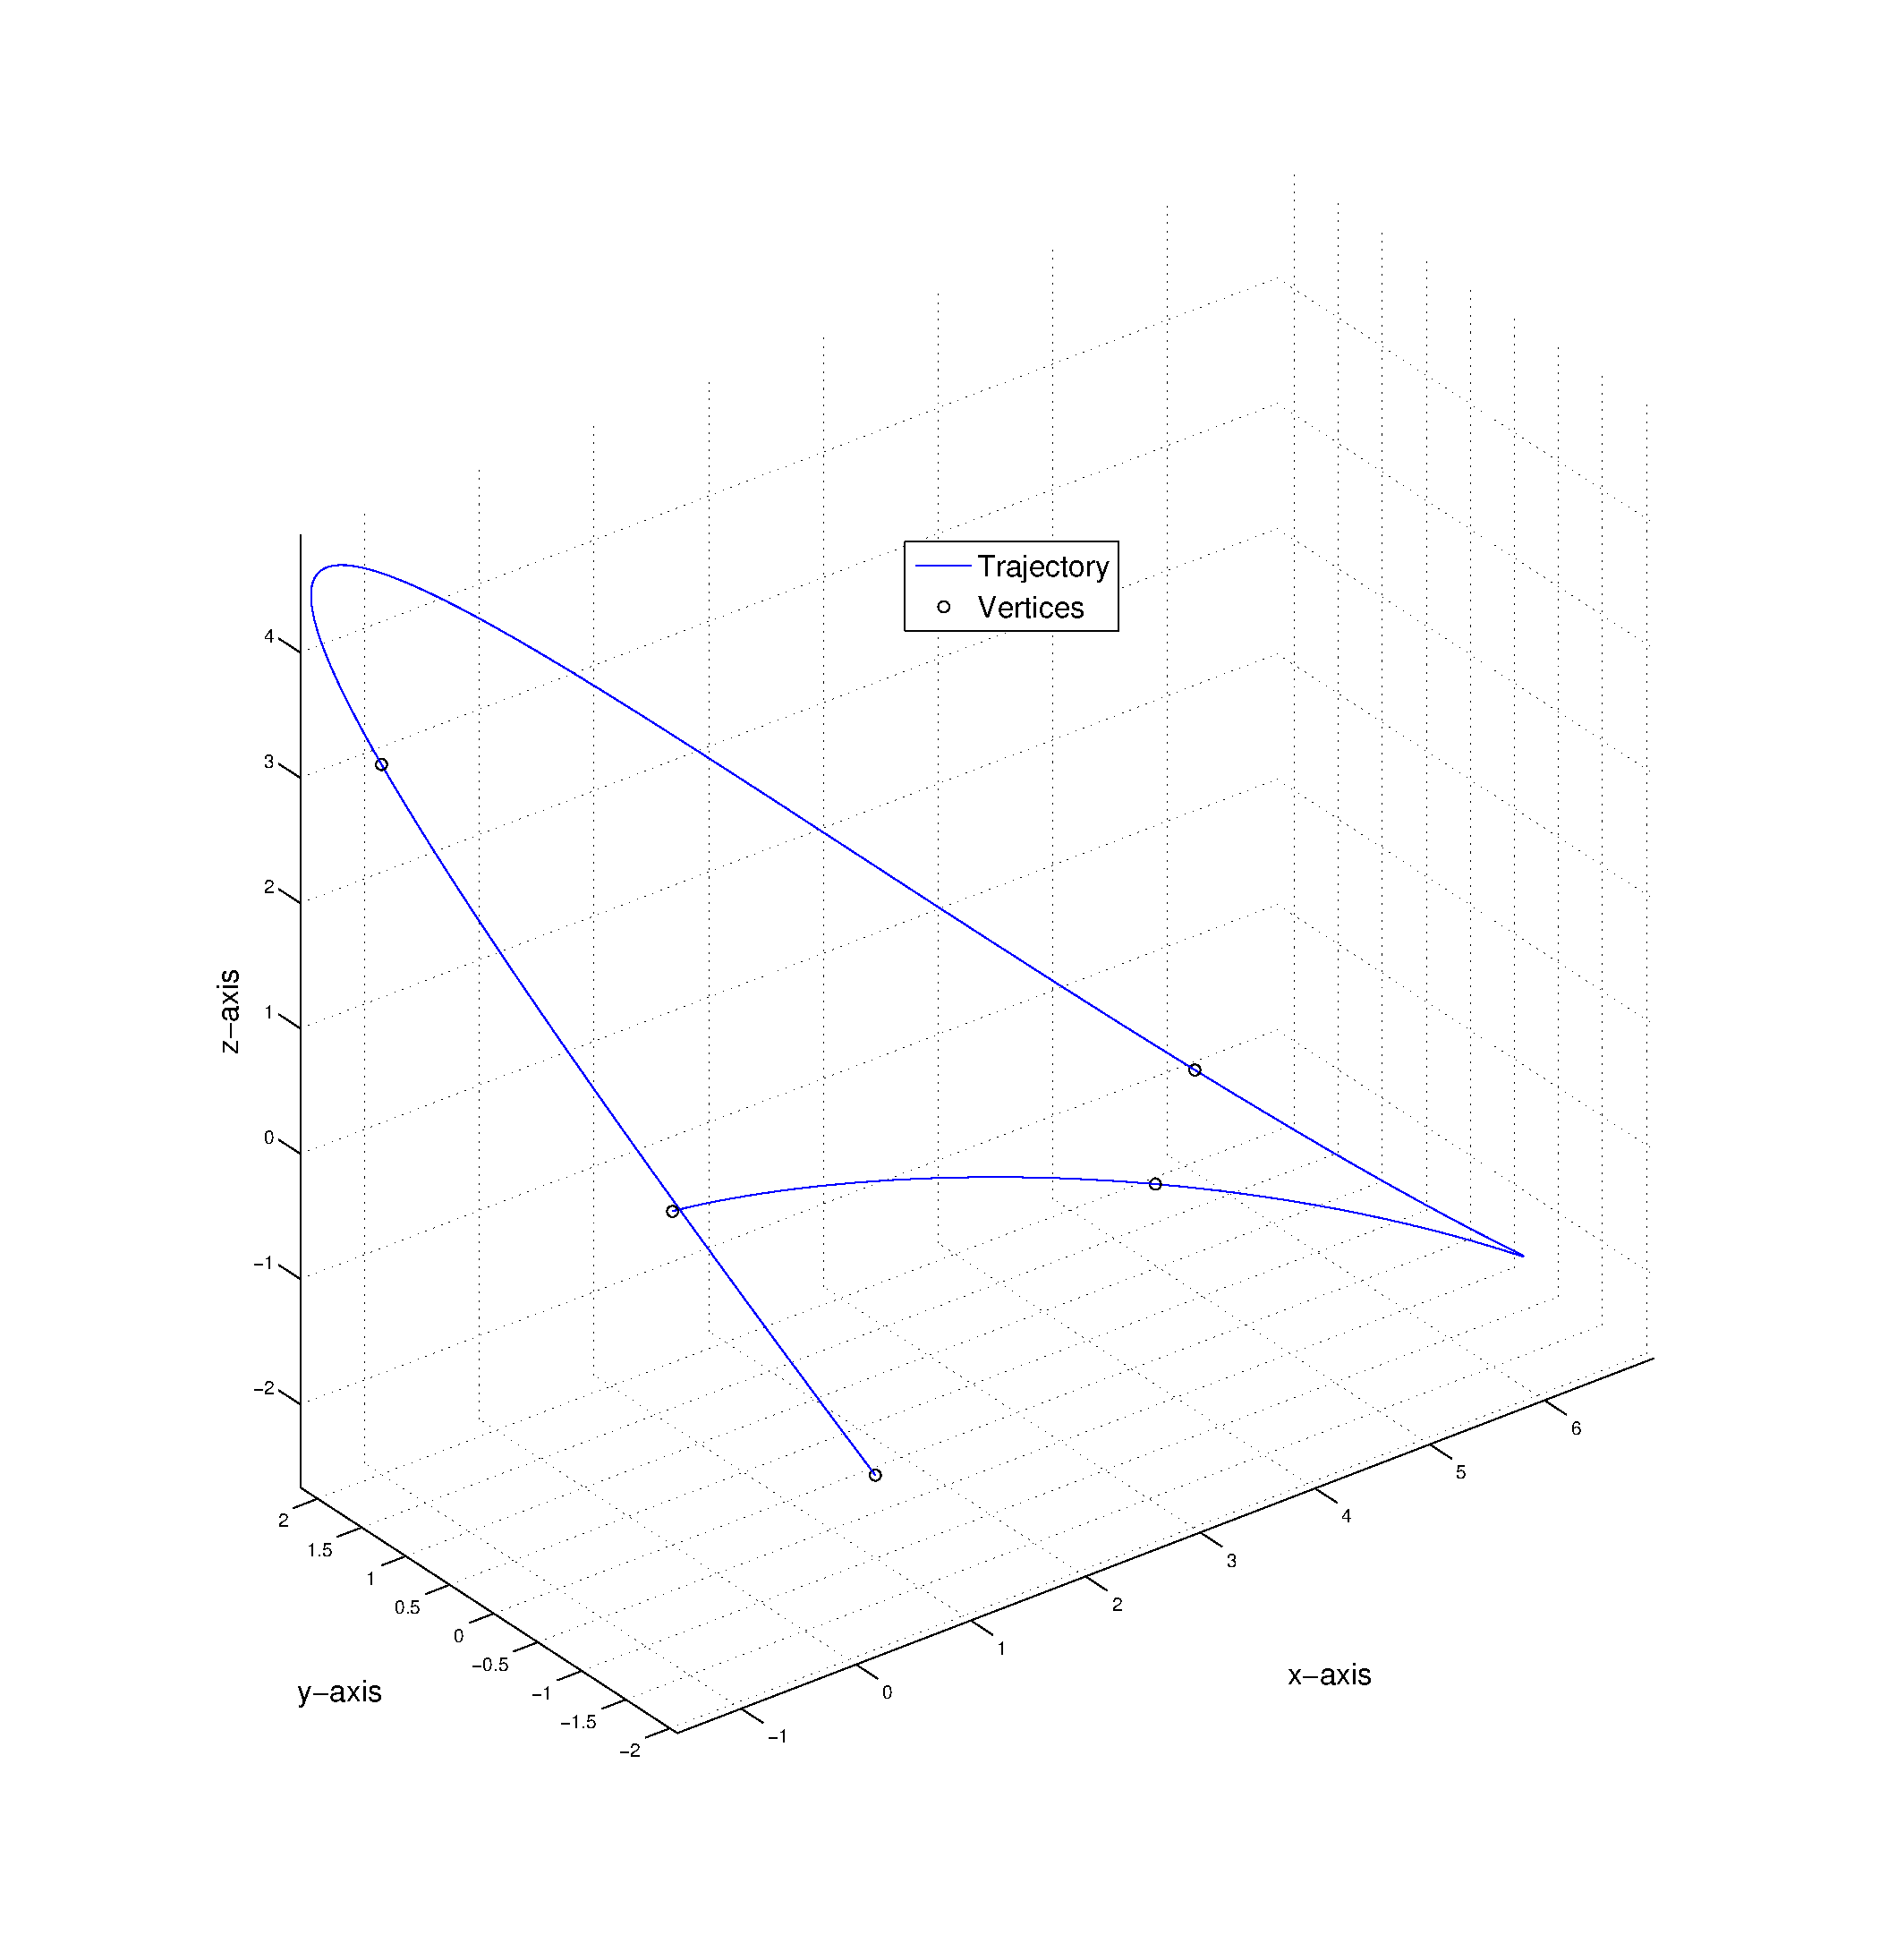
\includegraphics[trim = 36mm 30mm 33mm 30mm,clip,width=1\textwidth]{pics/4SegInitSpace.eps}
   \caption{3D plot of the initial trajectory with 4 segments. The start vertex is located at (0/0/0) and the trajectory proceeds counter-clockwise.}
   \label{pic:initiSpace} 
\end{figure}


Figure \ref{pic:initiSpace} depicts the initial trajectory (from figure \ref{pic:optimizedSolution4init}) in 3D space. Again, the vertices are marked as circles but now the time is no longer explicit readable. The start vertex is located at (0/0/0) and the trajectory proceeds counter-clockwise. The second segment (lower right corner) of the initial trajectory in figure \ref{pic:initiSpace} looks very sharp. Such sharp corners, accrued by the suboptimal segment time ratio, are undesirable if the UAV should fly a trajectory dynamically. \newline

By optimizing the ratio of the segment times, which is implicitly performed during the nonlinear optimization, the pathway of the trajectory gets smoother, i.e. no sharp corners exist in the optimized trajectory.\newline 
Figure \ref{pic:optiSpace} depicts the optimized trajectory (from figure \ref{pic:optimizedSolution4optik2000}) in 3D space. Especially the second segment of the optimized trajectory is now more suitable for a dynamic flight. In addition, the pathway in the region of the 4. vertex (in the upper left corner) is improved. The initial trajectory made a detour before passing the 4. vertex. This detour, accrued by the suboptimal segment time ratio, vanishes in the optimized trajectory.



\begin{figure}[H]
   \centering
   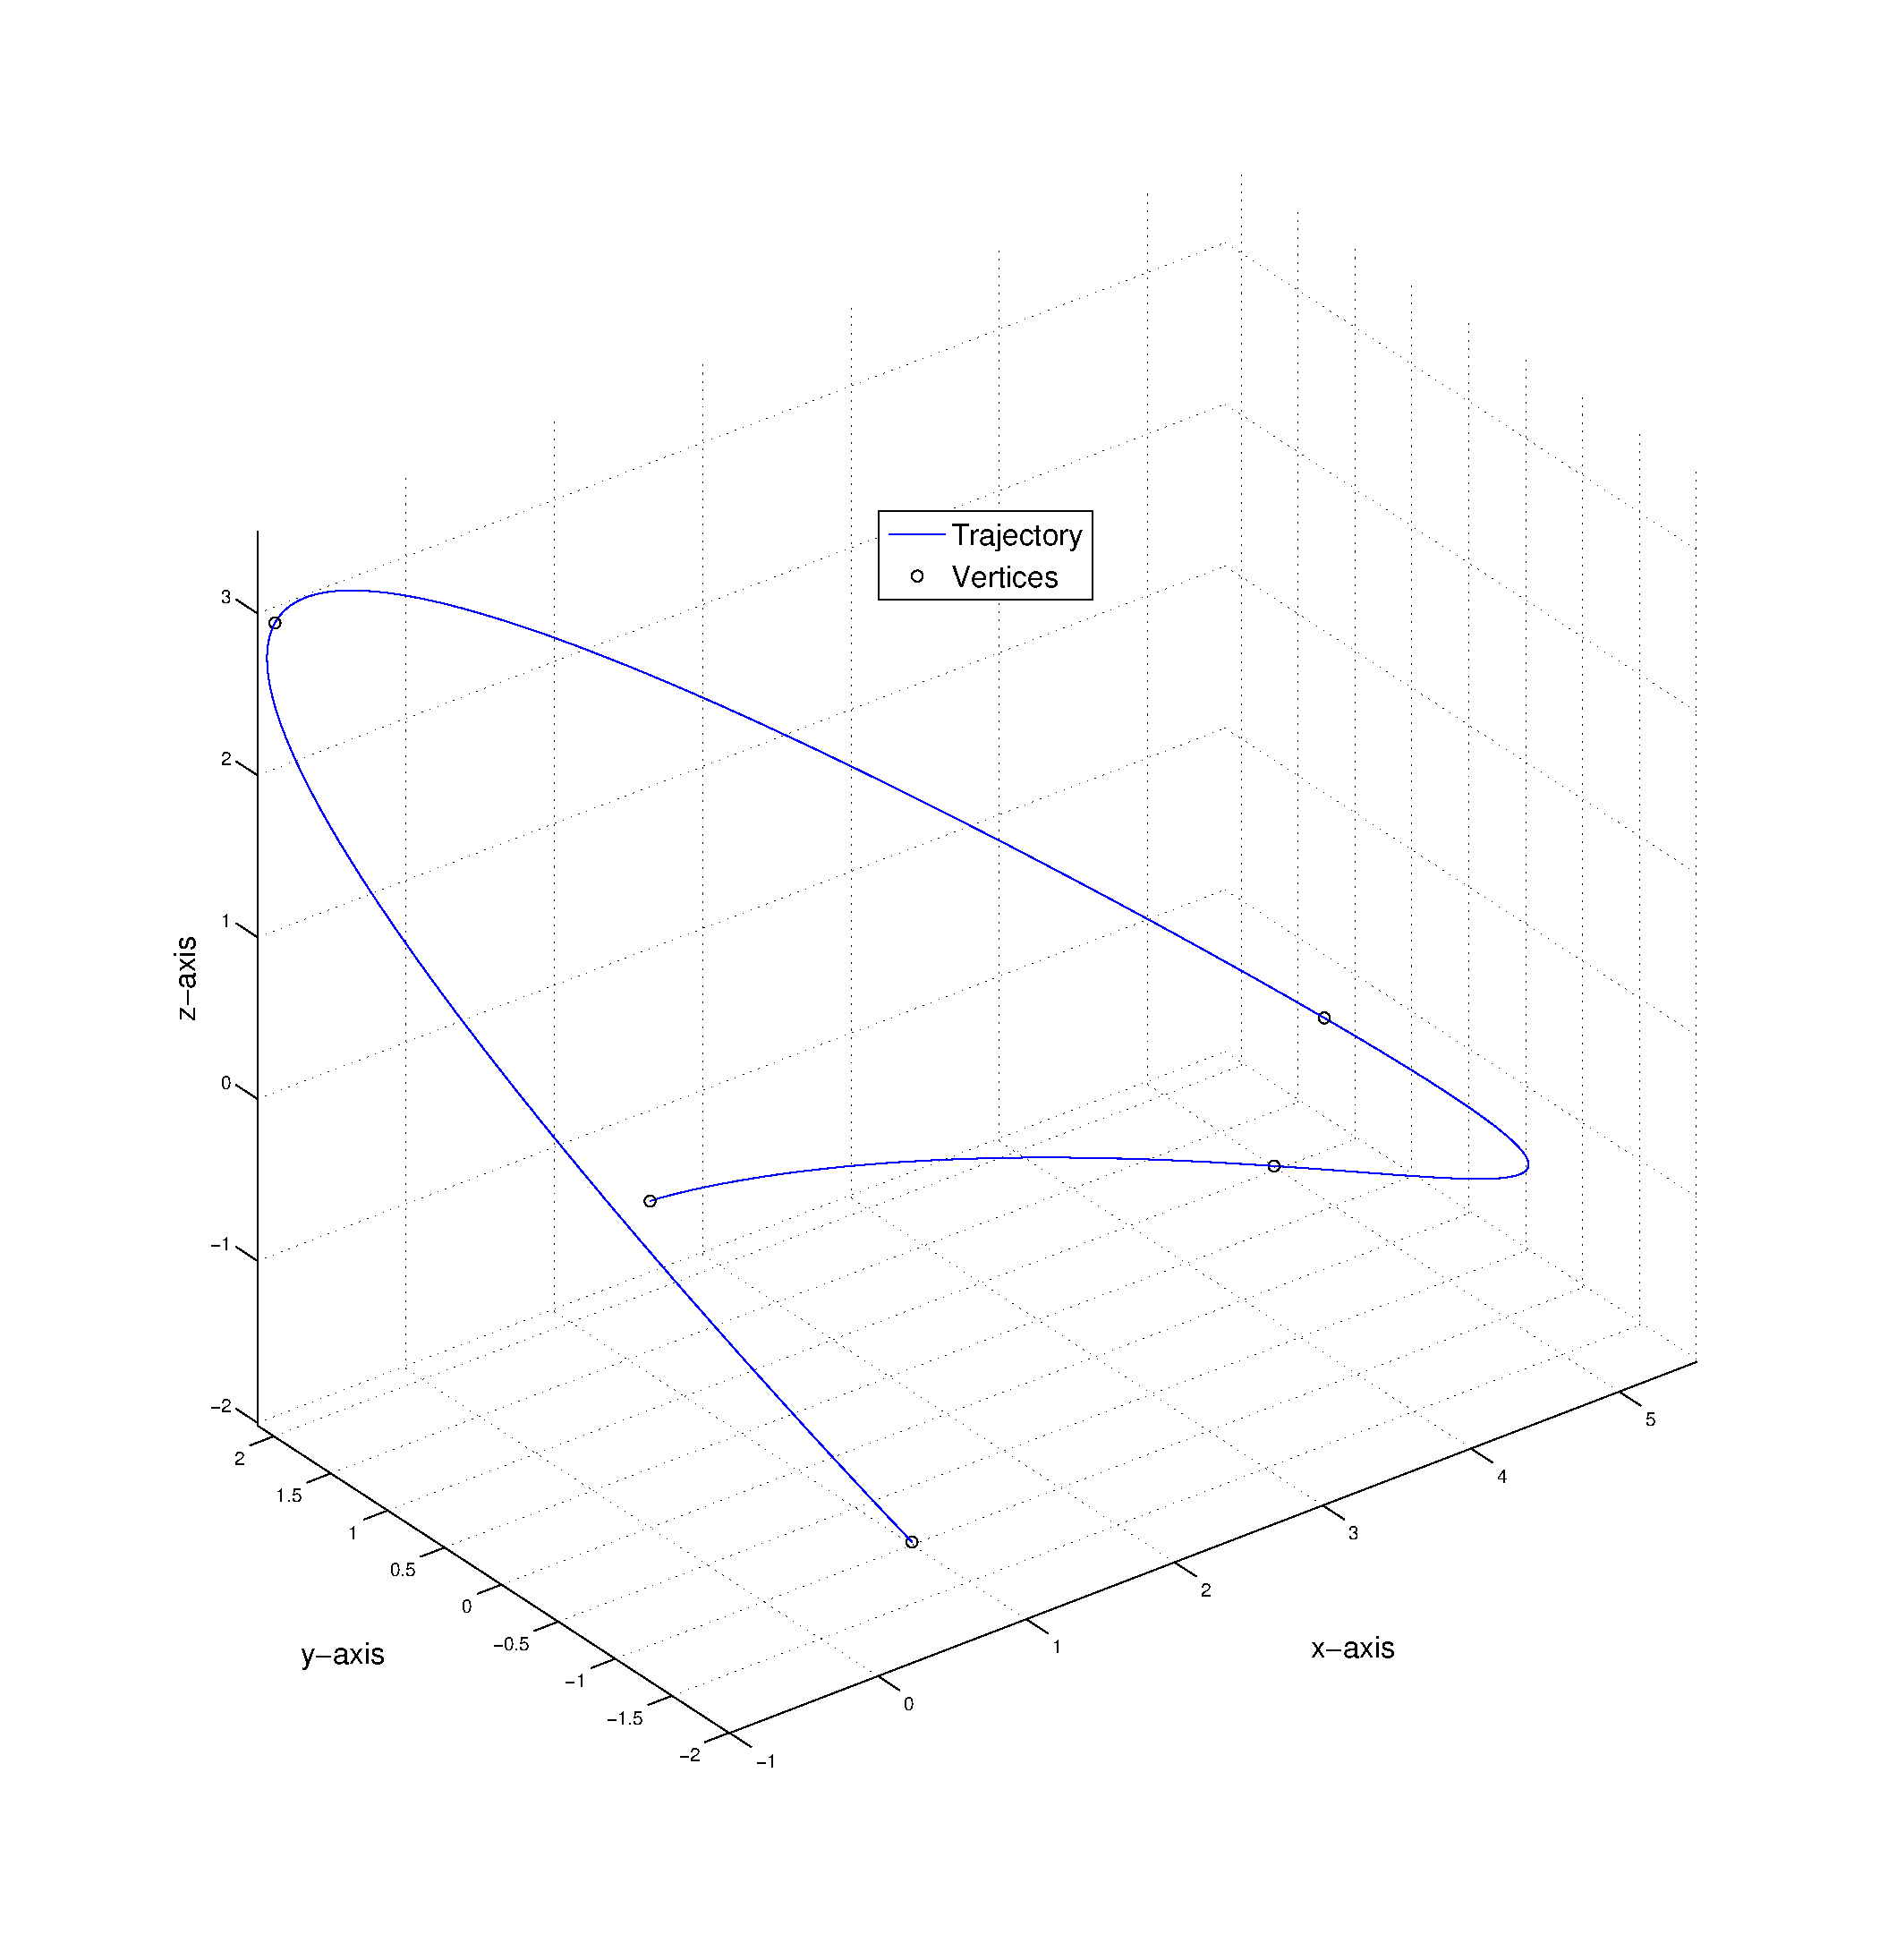
\includegraphics[trim = 30mm 30mm 33mm 30mm,clip,width=1\textwidth]{pics/4SegOptiSpace.eps}
   \caption{3D plot of the optimized trajectory with 4 segments. The start vertex is located at (0/0/0) and the trajectory proceeds counter-clockwise.}
    \label{pic:optiSpace} 
\end{figure}
\newpage


\section{NLopt}\label{sec:NLopt}

For all the nonlinear optimizations which were performed in the previous sections, \href{http://ab-initio.mit.edu/wiki/index.php/NLopt}{NLopt} \cite{NLopt}, an open-source library for nonlinear optimization, was applied. The optimization algorithm tries to minimize the cost function every iteration and needs parameters for termination condition in order to know when to stop.\newline
The termination condition of the optimization can be specified by the optimization variables as well as by the total cost. Generally, the termination conditions are formulated relative to the current value(s). For instance, if the relative termination condition for the total cost $J_{rel}$ is set to $0.01$ the optimization ends if the total cost changes less than one percent during an iteration. The relative termination condition for the optimization variables $x_{rel}$ is only fulfilled if all of the optimization variables change less than the threshold in one iteration.
Additionally, an absolute termination condition $x_{abs}$ can be applied to the optimization variables. This termination condition is only needed if one or several optimization variables are close to zero and the relative criteria therefore does not work properly. \newline 

Two additional options for termination condition are the limitation of the number of optimization iterations and the limitation of the duration of the optimization. All of these termination condition can be set simultaneously and the first condition which is fulfilled stops the optimization.
During the optimization the constraints on velocity and acceleration are checked every iteration. \newline

For the previous optimization problems only $J_{rel}$ was applied. This is the general case, since the other parameters are mostly used to intercept if the the cost function does not converge.










%Once the segment times are calculated, the initial snap minimized solution can be computed according to equation \ref{equ:dpstar}. The initial solution for a 3 dimensional problem with 4 segments is depict in figure \ref{pic:initialSolution}. The start of the trajectory is the origin of the Cartesian coordinate system (0/0/0). For both, start and goal state, the velocity, the acceleration, the jerk and the snap are fixed and set to zero. For all the other sampling points (vertices) the derivatives are unspecified. The Cartesian coordinates of the sampling points are chosen manually and are listed in the following table: 
%




%\begin{figure}[h]
%   \centering
%   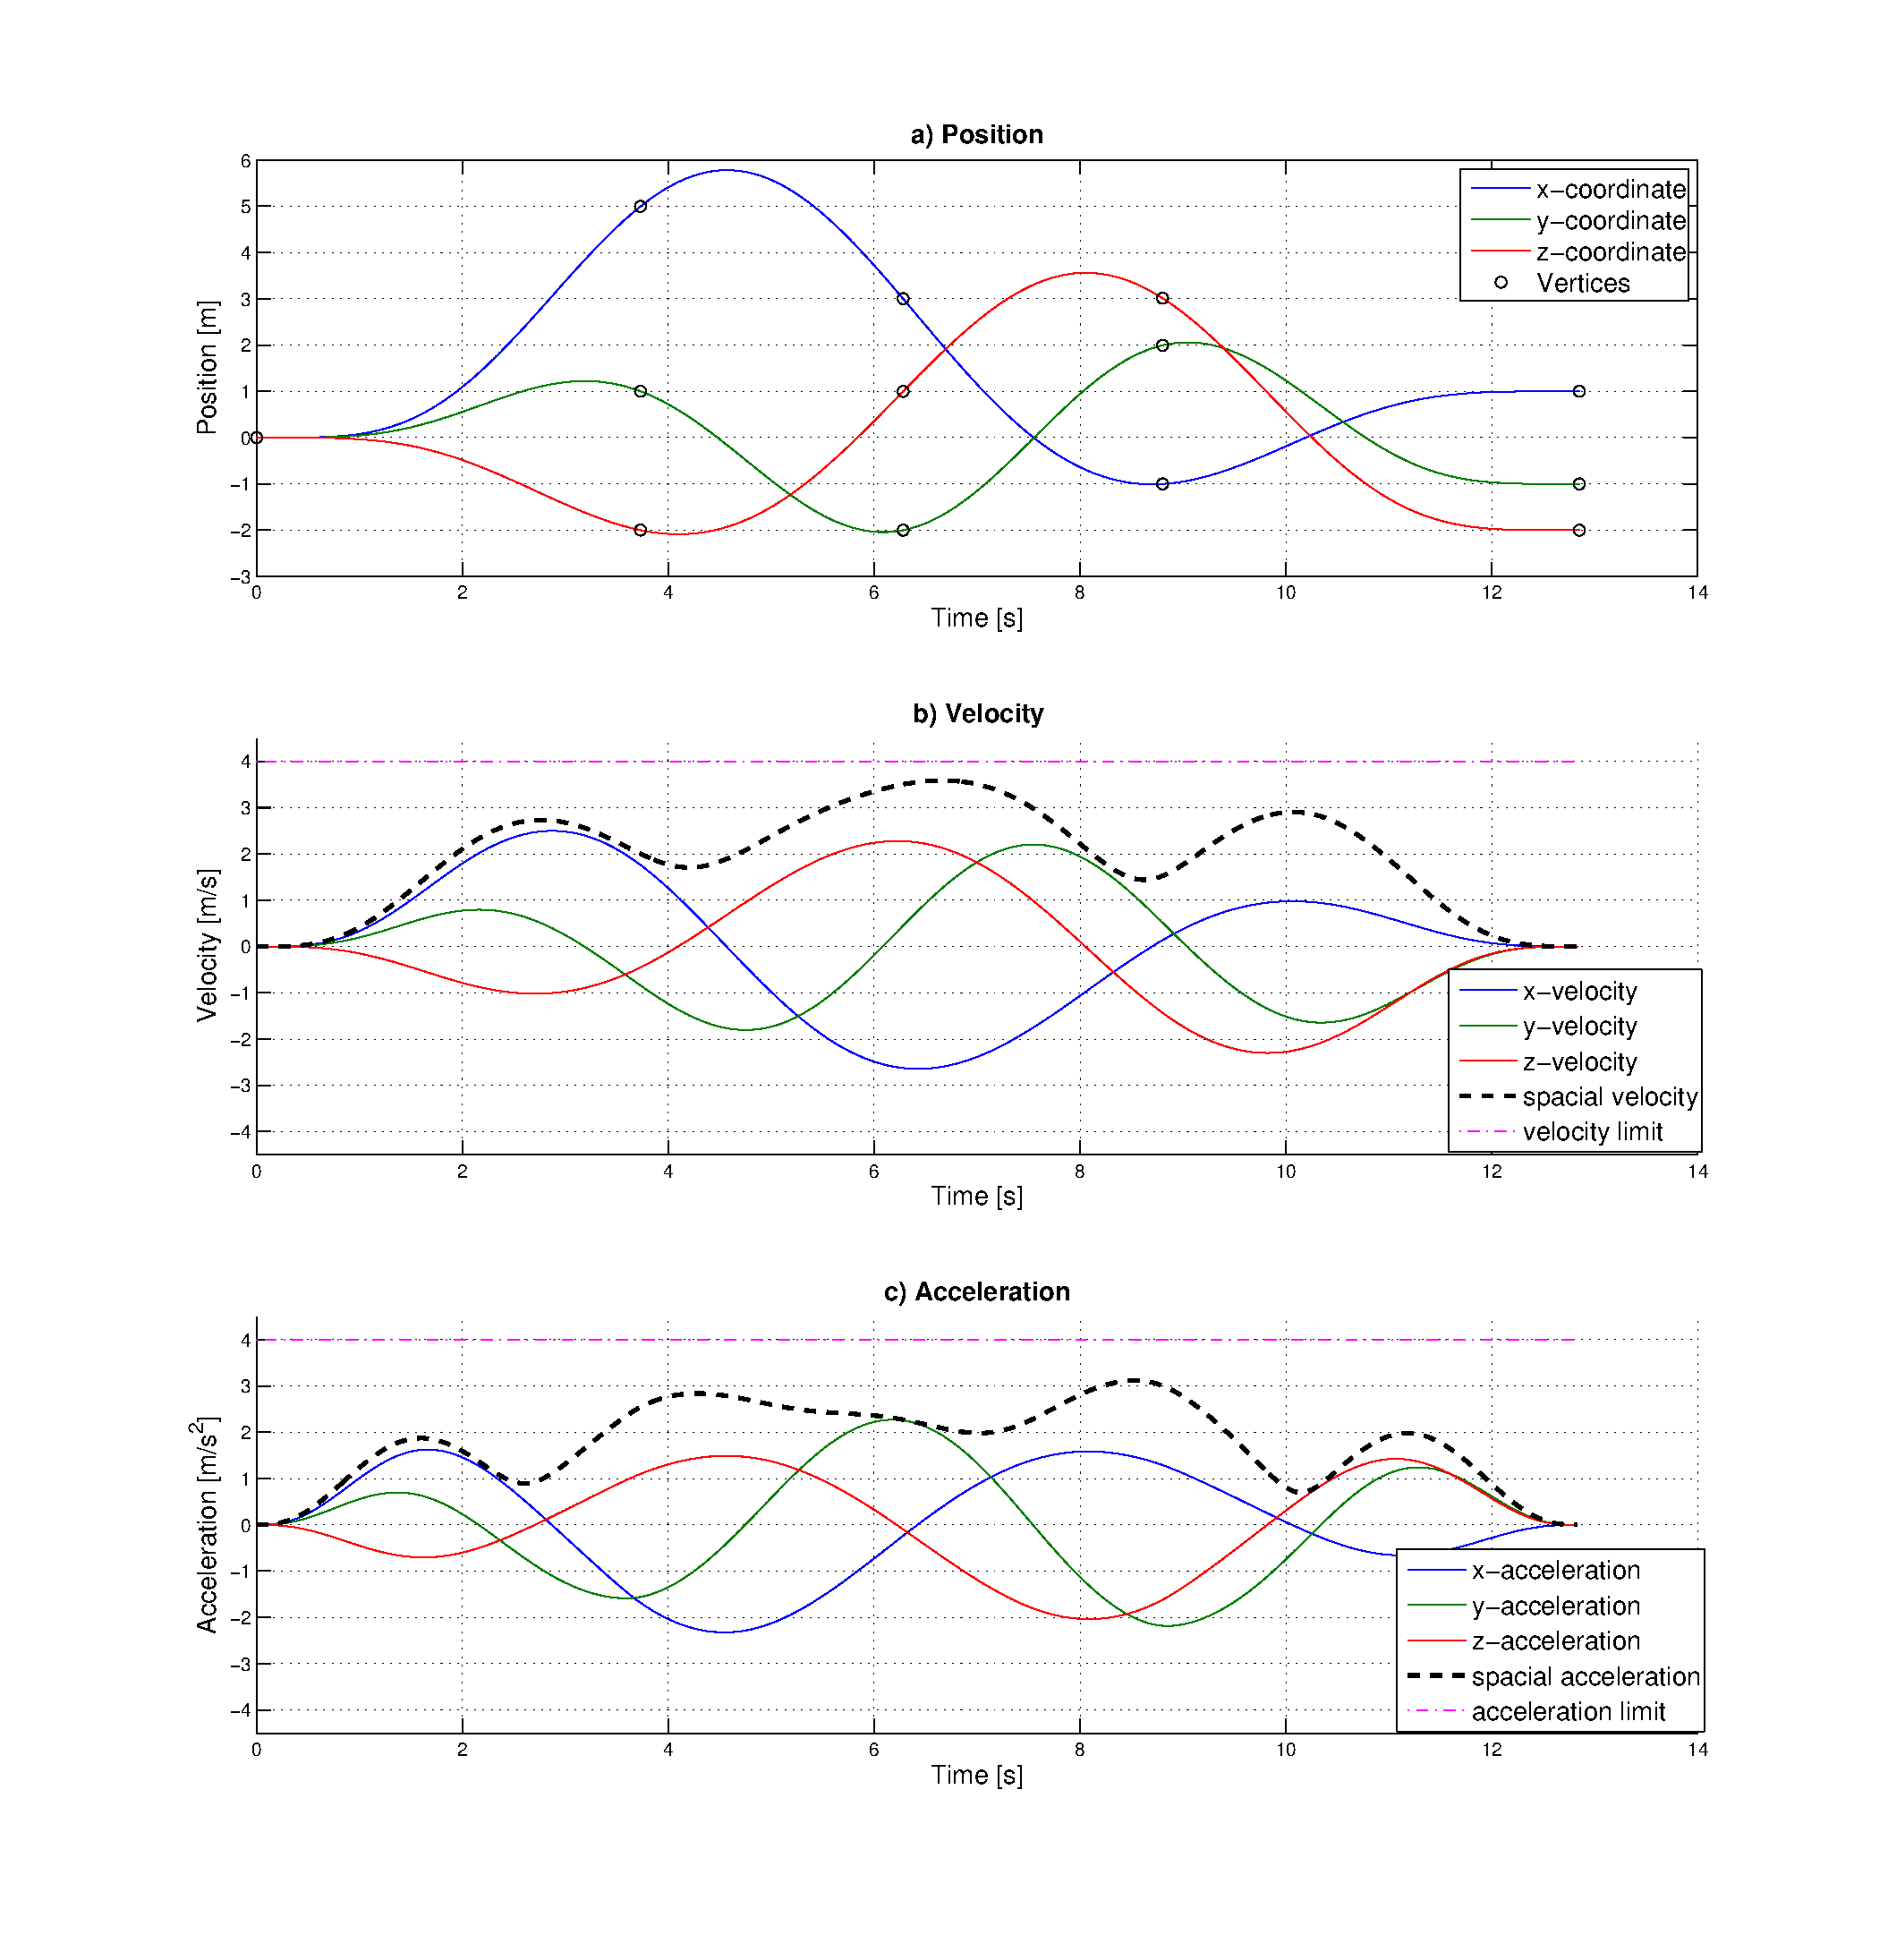
\includegraphics[trim = 35mm 20mm 30mm 35mm,width=1\textwidth]{pics/4SegOpti12s85k100.eps}
%   \caption{...................................................................................... ..... ............. . . . . ...................... ......... .........}
%\end{figure}
%
%
%
%
%





%\texttt{\begin{figure}[h]
%   \centering
%   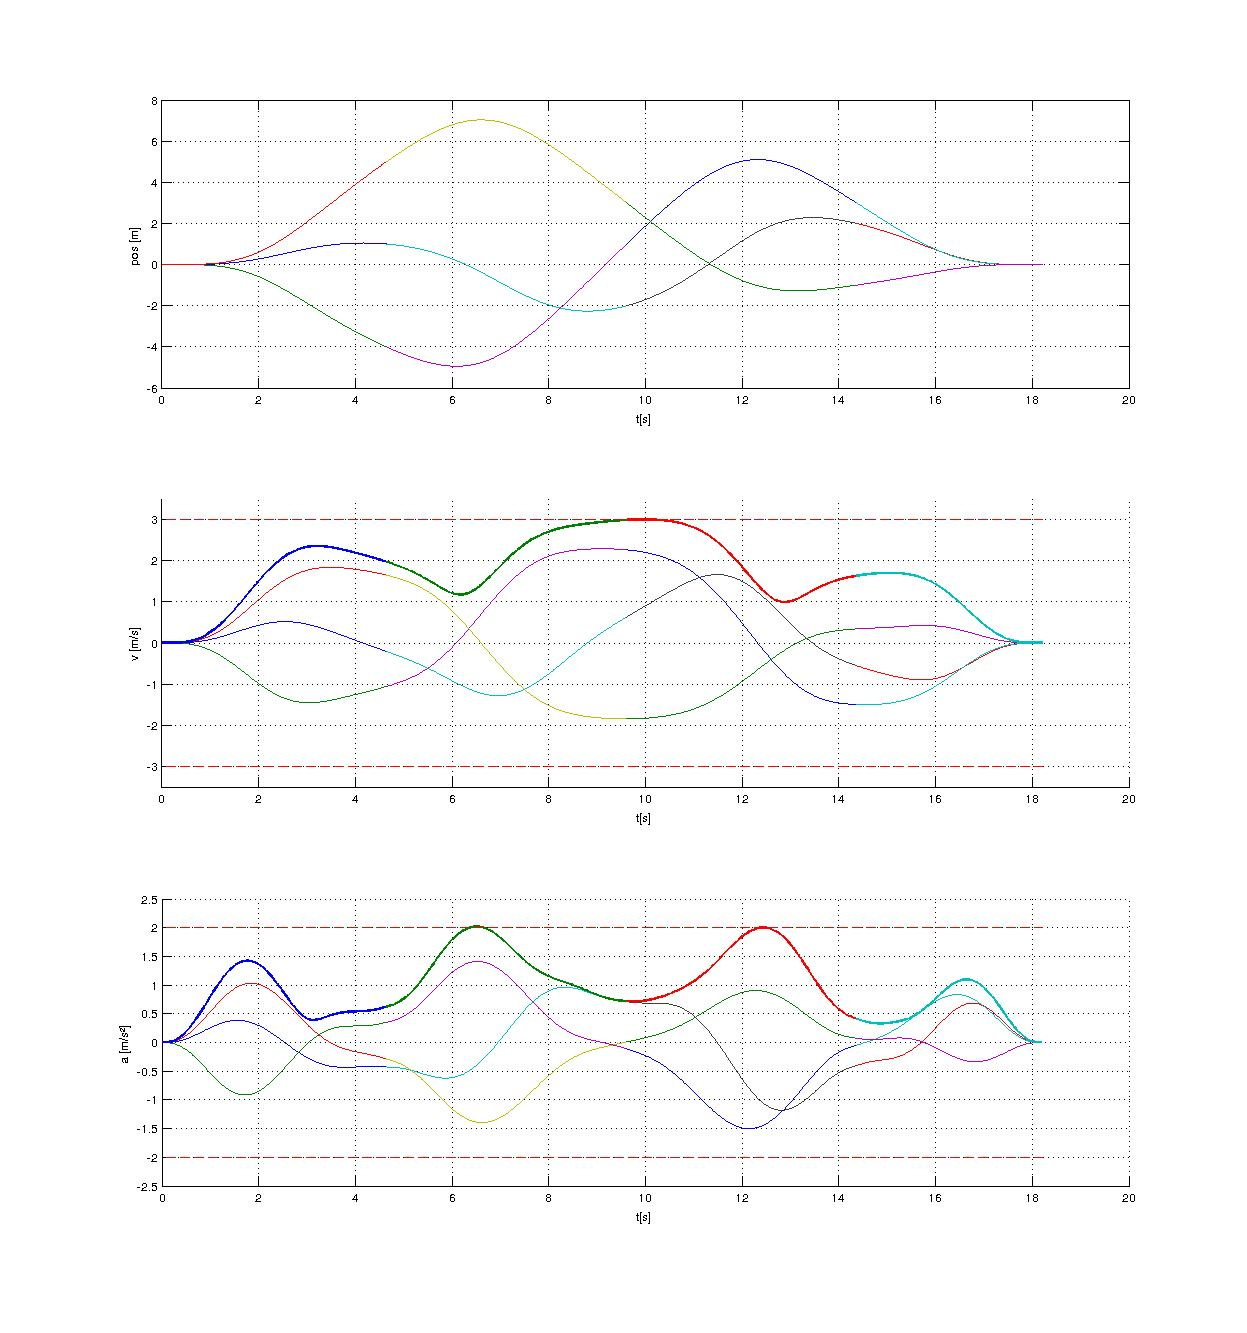
\includegraphics[width=1\textwidth]{pics/optimized.jpg}
%   \caption{Optimized solution of a trajectory with 4 segments: Plot a) shows the position (i.e. the Cartesian coordinates). Plot b) shows the velocity and plot c) the acceleration. A dashed graph represents the velocity respectively the acceleration in the three-dimensional space.}
%   \label{pic:optimizedSolution}
%\end{figure}}





%\begin{figure}[h]
%   \centering
%   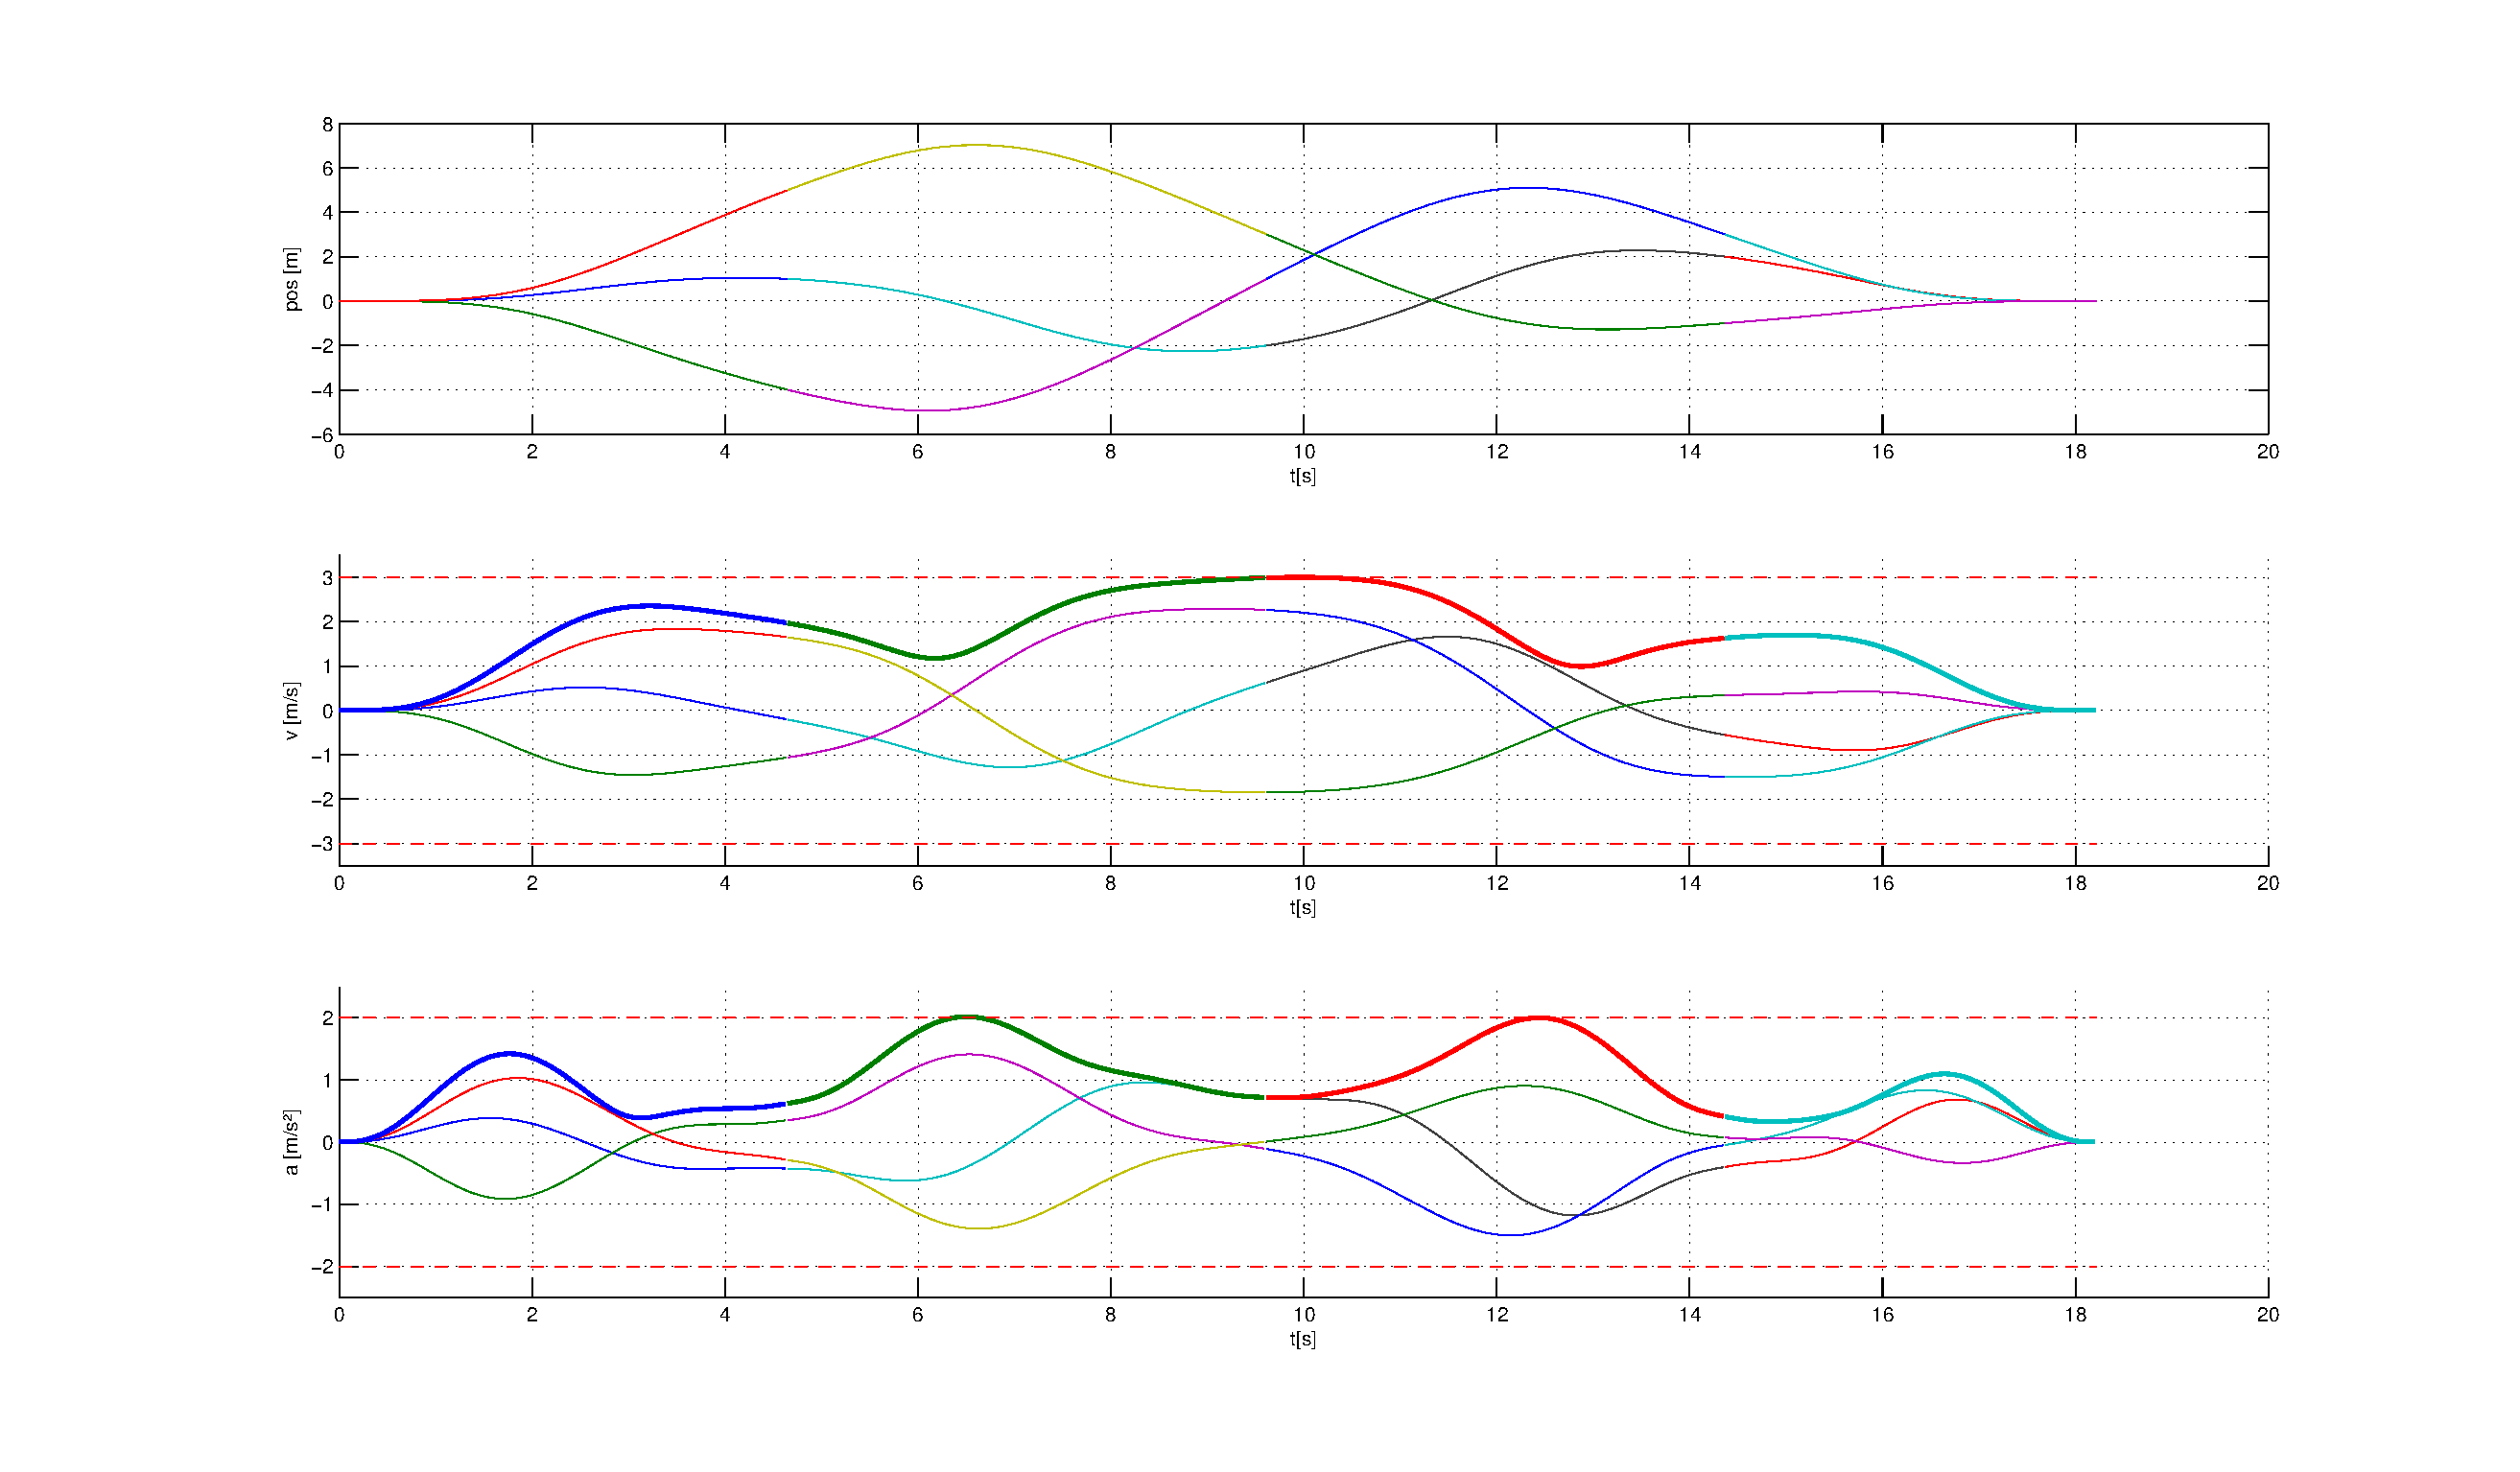
\includegraphics[width=1\textwidth]{pics/optimized.eps}
%   \caption{Ein Bild.}
%\end{figure}
%
%
%\begin{figure}[h]
%   \centering
%   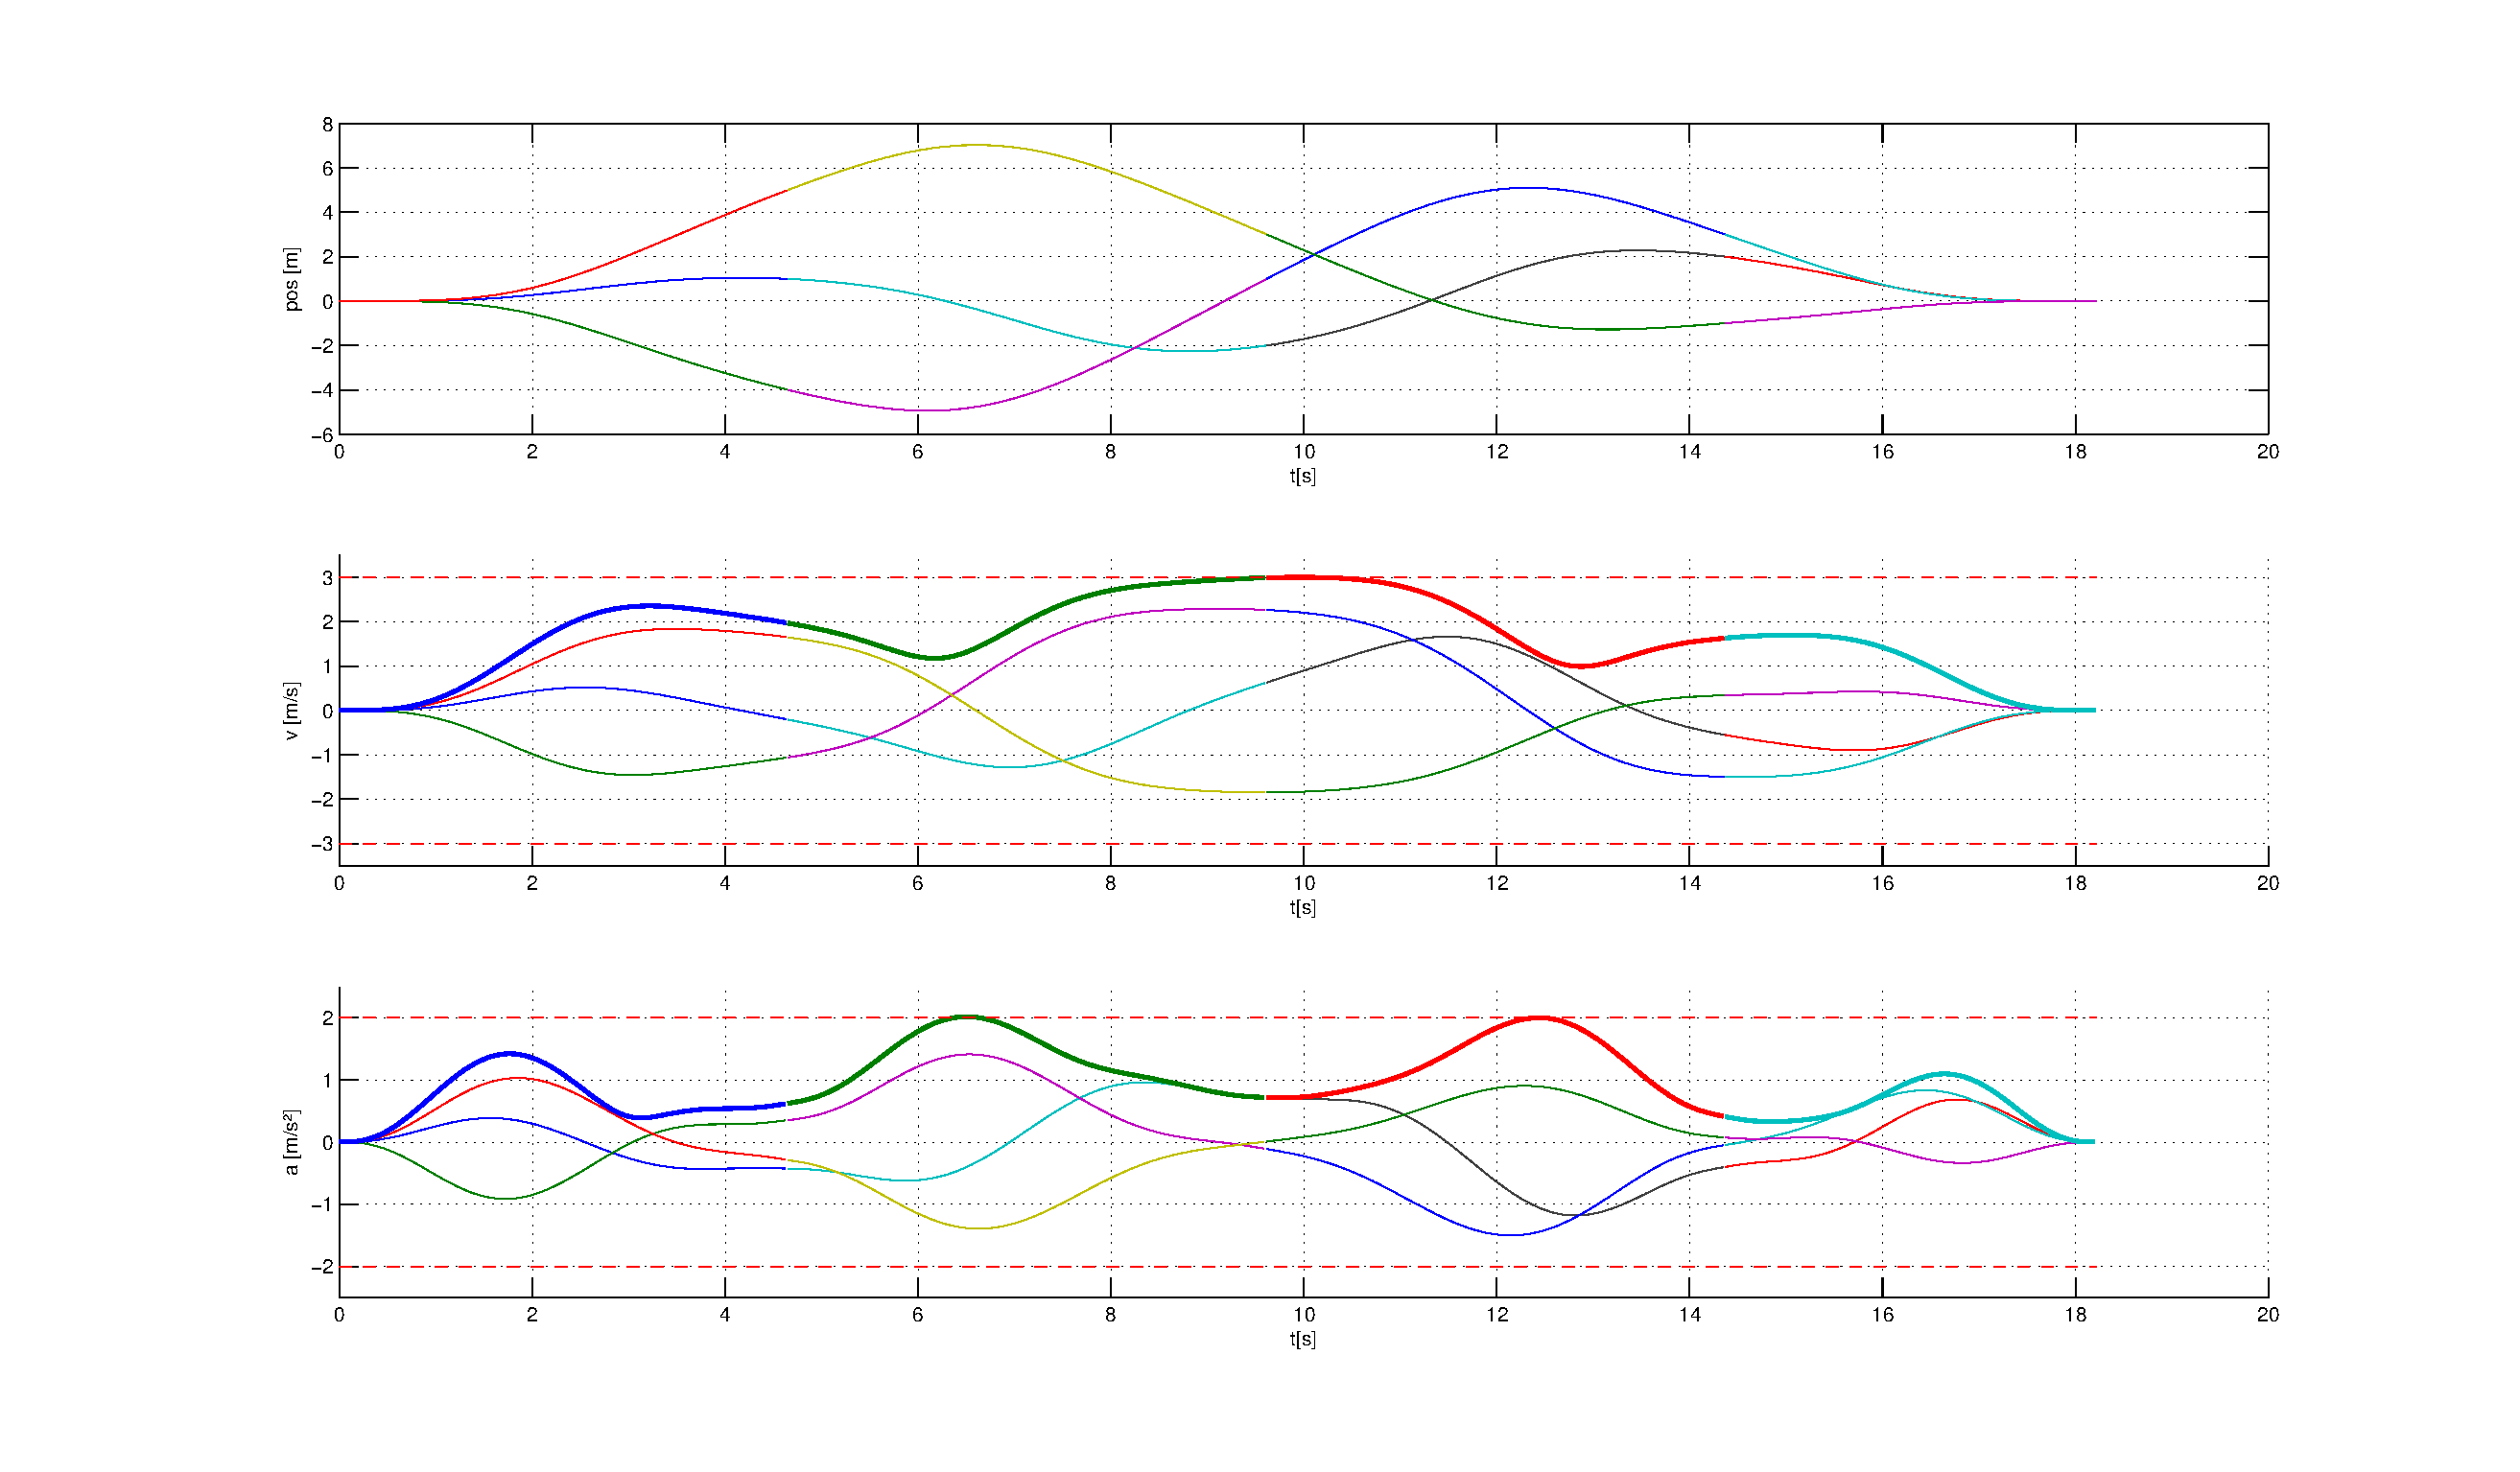
\includegraphics[scale=0.3]{pics/optimized.eps}
%   \caption{Ein Bild.}
%\end{figure}



%\begin{figure}[h]
%   \centering
%   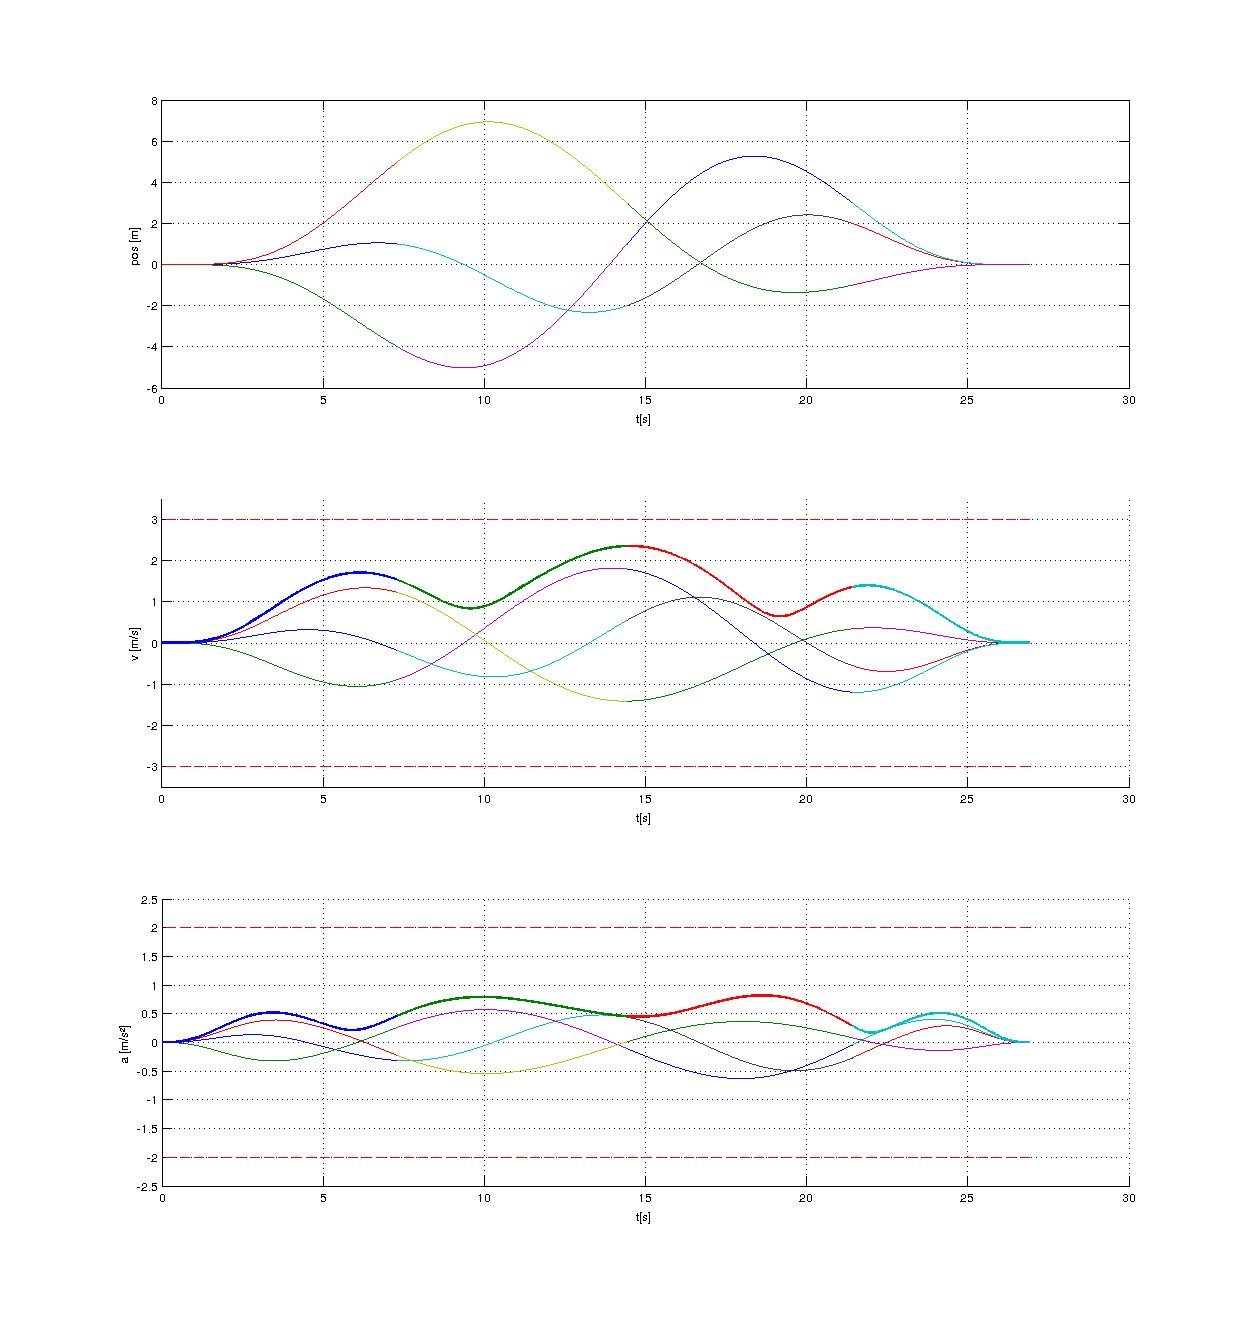
\includegraphics[width=1\textwidth]{pics/initial.eps}
%   \caption{Ein Bild.}
%\end{figure}

%\begin{figure}[h]
%   \centering
%   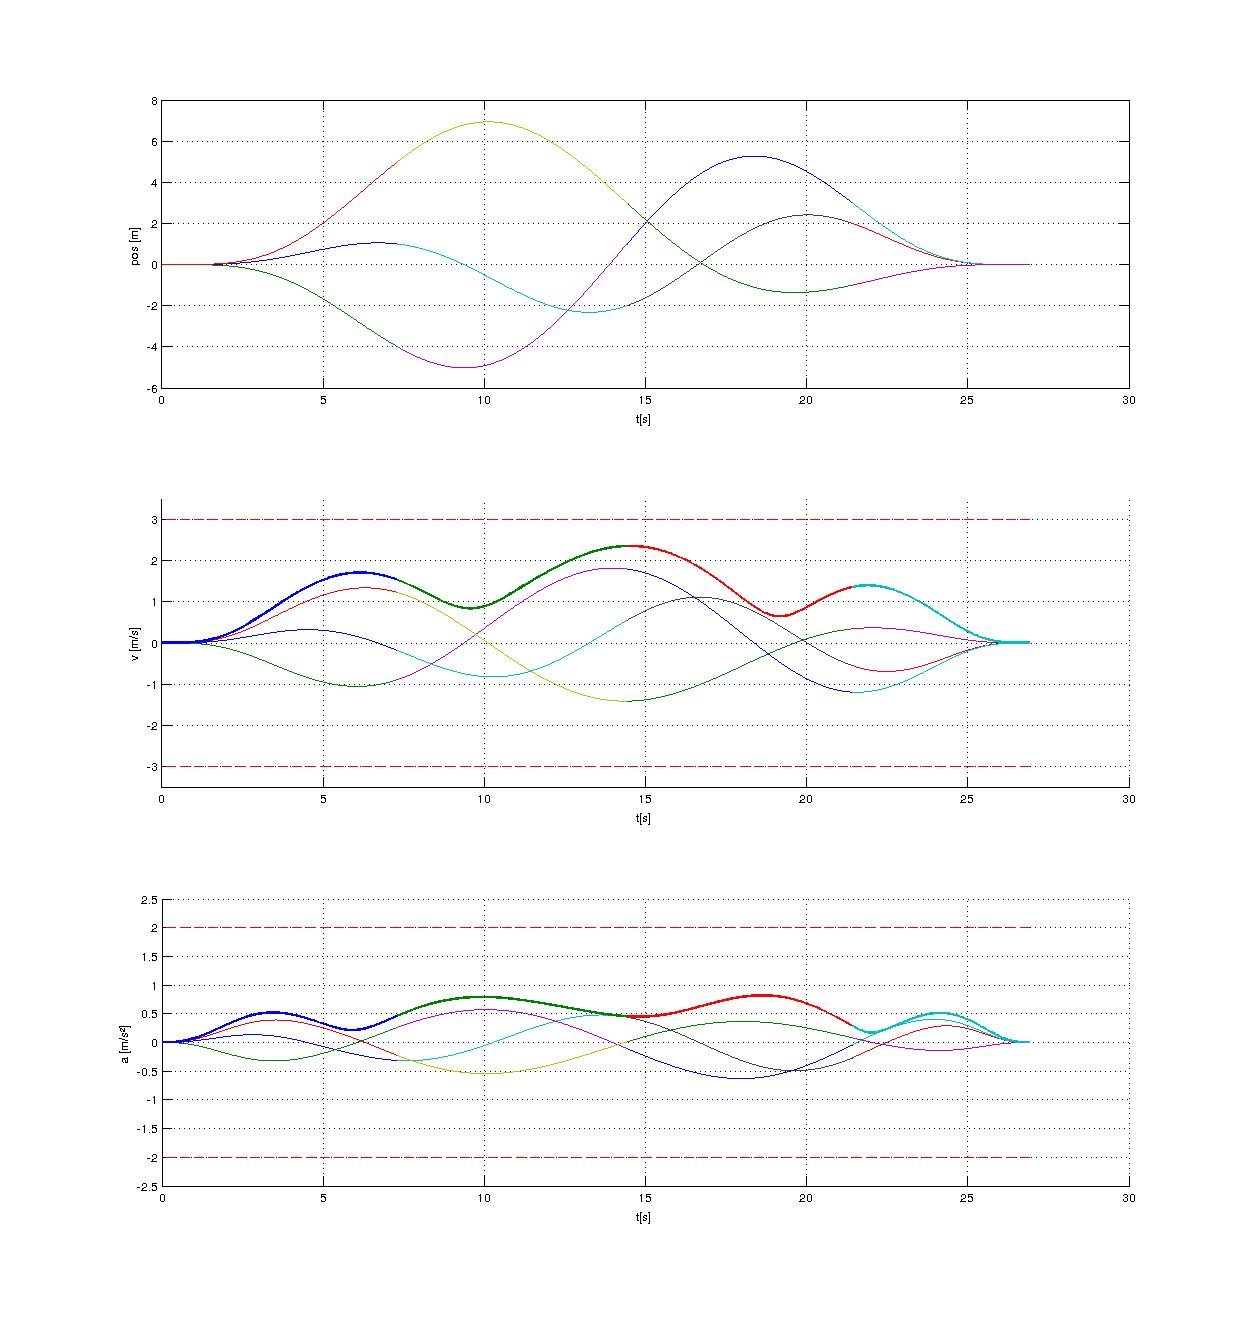
\includegraphics[scale=1]{pics/initial.eps}
%   \caption{Schematic of a rough foot surface.}
%   \label{pics:profile2}
%\end{figure}























